\documentclass{itetemplate_en-gb}

\usepackage{xparse}
\usepackage{multirow}
\usepackage{caption}
\usepackage{subcaption}
\usepackage{amssymb}
\usepackage{rotating}
\usepackage[nottoc, notlof, notlot]{tocbibind}
\usepackage{menukeys}

\usepackage{tikz}
\usetikzlibrary{arrows}
\usepackage{tikz-uml}

%% TODO glossary title
\makeglossary
\makeindex

\colorlet{linkcolor}{black!90!blue}
\colorlet{citecolor}{green!30!darkgray}


\hypersetup{
    linkcolor=linkcolor,          % color of internal links (change box color with linkbordercolor)
    citecolor=citecolor,        % color of links to bibliography
    filecolor=magenta,      % color of file links
    urlcolor=blue           % color of external links
}

\colorlet{punct}{red!60!black}
\definecolor{background}{HTML}{EEEEEE}
\definecolor{delim}{RGB}{20,105,176}
\colorlet{numb}{magenta!60!black}

\lstdefinelanguage{json}{
    basicstyle=\normalfont\ttfamily,
    	tabsize=4,
    numbers=left,
    numberstyle=\scriptsize,
    stepnumber=1,
    numbersep=8pt,
    showstringspaces=false,
    breaklines=true,
    frame=lines,
    backgroundcolor=\color{background},
    literate=
     *{0}{{{\color{numb}0}}}{1}
      {1}{{{\color{numb}1}}}{1}
      {2}{{{\color{numb}2}}}{1}
      {3}{{{\color{numb}3}}}{1}
      {4}{{{\color{numb}4}}}{1}
      {5}{{{\color{numb}5}}}{1}
      {6}{{{\color{numb}6}}}{1}
      {7}{{{\color{numb}7}}}{1}
      {8}{{{\color{numb}8}}}{1}
      {9}{{{\color{numb}9}}}{1}
      {:}{{{\color{punct}{:}}}}{1}
      {,}{{{\color{punct}{,}}}}{1}
      {\{}{{{\color{delim}{\{}}}}{1}
      {\}}{{{\color{delim}{\}}}}}{1}
      {[}{{{\color{delim}{[}}}}{1}
      {]}{{{\color{delim}{]}}}}{1},
}

% Usage:
% \includecode[language]{source file}{caption}{label}
\newcommand{\includecode}[4][h]{
	\lstinputlisting[float, caption=#3, escapechar=, language=#1, label=#4]{#2}
}
\DeclareDocumentCommand{\newdualentry}{ O{} O{} m m m m } {
  \newglossaryentry{gls-#3}{name={#5},text={#5\glsadd{#3}},
    description={#6},#1
  }
  \newacronym[see={[Glossary:]{gls-#3}},#2]{#3}{#4}{#5\glsadd{gls-#3}}
}

%% metadata.tex
%%
%% Metainformation for the document
%%
\subject{
	% the subject of your work e.g. Diploma, Großer Beleg ...
	Großer Beleg
}

\title{
	% the title of your works
	Graphical Support for the Design and Evaluation of Configurable Logic Blocks
}

\author{
	% Full name of the author
	Fredo Erxleben
}

\date{
	% the date of publication
	\today
}

\newcommand{\supervisingprof}{
	% the name of your supervising professor
	Prof. Dr.-Ing. habil. Rainer G. Spallek
}

\newcommand{\supervisor}{
	% the name of your supervisor
	Dr.-Ing. Thomas B. Preußer
}

\newcommand{\bornat}{
	% the authors date of birth
	30th\ April\ 1987
}

\newcommand{\bornin}{
	% the authors place of birth
	Blankenburg\,(Harz)
}

\newcommand{\matriculation}{
	%the authors matriculation number
	33\,00\,664
}

\newcommand{\makeabstract}{
	%% put your abstract here
	\paragraph{Abstract}
	Developing a tool supporting humans to design and evaluate \gls{clb}-based circuits requires a lot of know-how and research from different fields of computer science.
	In this work, the newly developed application \emph{q2d}, especially its design and implementation will be introduced as a possible tool for approaching \gls{clb} circuit development with graphical \gls{ui} support.
	Design decisions and implementation will be discussed and a workflow example will be given.
	
	\vspace{4cm}	
	
	\paragraph{Thanks to\dots}
	\begin{itemize}
	\renewcommand{\labelitemi}{\dots}
	\item \emph{Dr. Thomas Peußer}, for letting me occupy a chair in his office, providing a \emph{C/C++} interface for \gls{quantor} using his own parser \emph{wisent} and being a great supervisor.
	
	\item \emph{Dipl.-Inf. Marcus Hähnel}, who offered a lot of advice regarding proper \emph{C++} and \gls{qt}, did code reviews, beta tests and improved the applications build script to be more user friendly.
	
	\item \emph{(Soon to be Dipl.-Minf.) Paula Schöley}, for lengthy discussions about \glspl{ui}, human-machine interaction as well as human perception of shapes and colors. 

	\item \emph{my family and friends}, helping me to keep my feet on the ground

	\item \emph{Krümelchen}, helping me to keep my head in the clouds.
	\end{itemize}
} % !!! do not forget to fill theese in
%% glossary.tex
%%
%% Write down all your entries for your glossary here.
%% Abbreviations go to acronyms.tex
%%

%% --- C ---
\newdualentry{cbd}{CBD}{Component Behaviour Descriptor}{
The set of all \glspl{pcbd} referring to the same component context forms the holistic description of the components behaviour.
A formal definition can be found in section \ref{sec-definitions}.
}

%% --- D ---
\longnewglossaryentry{din}{name=DIN}{
	\emph{Deutsche Industrienorm}, German industrial standard.
}

%% --- G ---
\longnewglossaryentry{github}{name=GitHub}{
	A web-based provider for \emph{git}-repositories. The site features convenient tools for many standard tasks that come with the management of projects and repositories.
	The official website can be found at \url{www.github.com}.
}

%% --- P ---
\newdualentry{pcbd}{pCBD}{partial Component Behaviour Descriptor}{
A boolean formula, containing a subset of the node and configuration variables of a component context, is called a \emph{partial} \gls{cbd}.
All \glspl{pcbd} of a component form the \gls{cbd}.
See also section \ref{sec-definitions} and the entry for \gls{gls-cbd}.
}

%% --- Q ---

\longnewglossaryentry{qt}{name=Qt}{
A framework based on the \emph{C++} programming language. 
It extends the language features of \emph{C++} by the use of a meta-compiler and and thereby enables amongst other things the use of introspection and signal-slot concepts.
Common \glspl{os} like \emph{Linux}, \emph{Windows}, \emph{OS\,X} or \emph{Android} are well supported.
Furthermore, libraries are offered for a lot of standard tasks like the abstraction of graphical \glspl{ui}, \gls{json}-parsing, device interaction, unit testing\dots
\glspl{ide} specialized for the development with \emph{Qt} exist and provide support for the visual design of \glspl{ui} and internationalisation of developed applications while also integrating user-defined external tools and workflows.
The official website can be found at \url{qt-project.org}.
}

\longnewglossaryentry{quantor}{name=Quantor}{
An open-source solver for \gls{qbf} problems.
It was developed by the Johannes-Kepler University of Linz and is written in \emph{C}.
Internally, the \gls{sat} solver \emph{picosat} is employed.
Both tools can be found at \url{fmv.jku.at/quantor} and \url{fmv.jku.at/picosat} respectively.
}

\longnewglossaryentry{qucs}{name=Qucs}{
The \emph{Quite universal circuit simulator} is an open source tool for the visual design and simulation of analogous circuits.
Recent development has expanded it to offer basic design and evaluation features for digital components as well.
An exhaustive description can be found at \cite{Qucs:base} in combination with \cite{Qucs:devel}.
The official website can be found at \url{qucs.sourceforge.net}
}

\longnewglossaryentry{}{name=}{

} % define all entries for your glossary in there
%% acronyms.tex
%%
%% Define all your abbreviations in this file.
%%

%% --- C ---
\newacronym{cmux}{CMux}{configurable multiplexer}
\newacronym{clb}{CLB}{configurable logic block}
\newacronym{cnf}{CNF}{clause normal form}
\newacronym{cpld}{CPLD}{complex programmable logic device}

%% --- F ---
\newacronym{fpga}{FPGA}{field-programmable gate-array}

%% --- H ---
\newacronym{hdl}{HDL}{hardware design language}

%% --- I ---
\newacronym{ide}{IDE}{integrated development environment}

%% --- J ---
\newacronym{json}{JSON}{JavaScript object notation}

%% --- L ---
\newacronym{lsb}{LSB}{least significant bit}
\newacronym{lut}{LUT}{lookup table}

%% --- M ---
\newacronym{msb}{MSB}{most significant bit}

%% --- O ---
\newacronym{os}{OS}{operating system}

%% --- Q ---
\newacronym{qbf}{QBF}{quantified boolean formula}

%% --- S ---
\newacronym{sat}{SAT}{satisfiability}
\newacronym{svg}{SVG}{scalable vector graphics}

%% --- U ---
\newacronym{ui}{UI}{user interface}
\newacronym{uml}{UML}{unified markup language}

%% --- X ---
\newacronym{xml}{XML}{extended markup language} % define all your acronyms in there

%
% The document itself
%
\begin{document}

\chapter{Introduction}

	\section{Forethoughts}

	\paragraph{Problem Statement}
	The aim of this work is the creation of a tool that can support hardware designers in evaluating the capabilities of \glspl{clb}.
	To achieve this, it is necessary to find ways of easily modelling configurable components using a graphical \gls{ui}.
	It is further required to offer a method to specify the intended behaviour of the whole design, at which point the tool should evaluate whether this specification can be implemented by the \gls{clb}, and by which configuration.
	

	\paragraph{Outline of the Solution}
	Initial research made clear that so far no tool exists for supporting this kind of \gls{clb} evaluation in a user friendly way.
	Attempts to extend already existing projects also proved to be difficult.
	As a consequence, a new application called \emph{q2d} was designed and implemented for the outlined purpose.
	It supports project management, \gls{clb}-based circuit design and the evaluation of such.
	The user is presented with an appealing graphical \gls{ui} and can create custom component types quickly, requiring only simple means.
	
	\paragraph{Involved Areas of Computer Science}
	In addition to the area of design and engineering of large-scale integrated circuits, several other fields of computer science are involved in creating an application capable of dealing with the posed task.
	As a result, the work at hand might also be worth reading for audiences engaged in these particular areas:
	
	\begin{description}
		\item[Computational Logic] is involved when discussing the theoretical background of the problem and solving the resulting \gls{qbf} problem in section \ref{sec-theoretical-background}.
		\item[\Gls{ui} Engineering] will be discussed largely in sections \ref{sec-ui-ergonomics}, \ref{sec-visualization-aspects} and \ref{sec-basic-interaction} where the presentation of information and user interaction will be discussed,
		\item[Software Engineering] comes in mostly during the design phase, when the choice of tools and the internal program structure is explained in sections \ref{sec-languages-frameworks}, \ref{sec-model-design} and its implementation in chapter \ref{sec-chapter-implementation}. 
	\end{description}

	\paragraph{Application Use Cases}
	The resulting application will operate on the register transfer level.
	It is designed to help the user focus on the design task he wishes to perform without distracting him with details regarding the concrete physical implementation of specific circuit elements.
	Therefore, \emph{q2d} is best suited to develop, test and explain concepts of configurable circuit designs and demonstrate their flexibility and limits.
	%TODO q2d logo	
	
	\section{Theoretical Background}
	\label{sec-theoretical-background}
	
	When looking at the posed problem from a mathematical perspective, it becomes clear that the solving of a \gls{qbf} problem is required.
	Intuitively speaking, the designed circuit and its components are to be described by boolean formulae. 
	For those, an interpretation is to be found, which lets all formulae become true.
	As such a satisfying interpretation defines suitable values for the configurable circuit elements, it will be called a \emph{configuration}.

\subsection{Definitions}
	\label{sec-definitions}
	
	For simplicity, a shorthand notation for the set of boolean values will be used as provided in equation \ref{eqn-define-Bool}.
	
	\begin{equation}
		\label{eqn-define-Bool}
		\mathbb{B} := \lbrace \bot, \top \rbrace
	\end{equation}

	When talking about circuits, the need to distinguish its elements from each other arises, since each of them establishes its own \emph{context}.
	This will be achieved by marking symbols referring to circuit element $\epsilon$ with the index $\epsilon$.
	If no index is given, the symbol refers to the circuit as a whole.
	This will also be referred to as the \emph{global context}.

	Further, it is useful to define three disjunct sets of variables. 
	Each of these sets has a distinct semantic meaning.
	
	\begin{description}
		\item[$C_\epsilon$] Configuration variables represent programmable bits that define the temporary specific behaviour of an element.
		
		\item[$N_\epsilon$] Node variables represent the interfacing points of components that serve as ports for interconnecting the overall circuit.
		
		\item[$X$] Input variables stand for the outside connections of the whole circuit that are driven arbitrarily during the circuit's operation by the surrounding world.
	\end{description}
	
	Let a \gls{pcbd} be given as a boolean formula on a set of configuration and node variables as in equation \ref{eqn-define-fsmall}.

	\begin{equation}
		\label{eqn-define-fsmall}
			f_{\epsilon, i}\left( V_\epsilon \right)
		\left|
			\begin{array}{l}
			V_\epsilon \subseteq \left( C_\epsilon \cup N_\epsilon \right) \\
			i \in \left[0,n\right); \, n \in \mathbb{N}
			\end{array}
		\right.
	\end{equation}

	An arbitrary large set of \glspl{pcbd} can be used to describe the behaviour of a single circuit element such as a component or a wiring.
	All those \glspl{pcbd} are combined in equation \ref{eqn-define-F-epsilon} into a set describing the whole circuit elements behaviour, called the \gls{cbd}.
	
	\begin{equation}
		\label{eqn-define-F-epsilon}
			F_\epsilon := \bigcup_n f_{\epsilon, n} \left( V_\epsilon \right)
	\end{equation}	
	
	% N, C, F form context of \epsilon	
	For any given element $\epsilon$, its \emph{local context} is defined in equation \ref{eqn-define-box-epsilon} as
	
	\begin{equation}
		\label{eqn-define-box-epsilon}
		\Box_\epsilon := \left(C_\epsilon, N_\epsilon, F_\epsilon \right)
	\end{equation}
	
\subsection{Expressing Connections between Circuit Elements}
	In the case of node variables, it may occur that two elements effectively refer to the same node.\footnote{
		For example, one might think of a wire that is connected to the port of a component.	
	}
	Then, given the existence of two elements $\epsilon_a$ and $\epsilon_b$ sharing the same node, this common node can be expressed as a boolean formula $\sigma_{a, b}$. 
	
	\begin{equation}
	\sigma_{a, b} = 
	\left\lbrace
	n_a \Leftrightarrow n_b
	\vert
		n_a \in N_{\epsilon_a} \wedge 
		n_b \in N_{\epsilon_b} \wedge 
		\, \text{$n_a$ and $n_b$ are connected}
	\right\rbrace
	\label{eqn-define-sigma}
	\end{equation}
	
	Note that the equivalence can be transformed as shown in equation \ref{eqn-resolve-equivalence}. 

	\begin{equation}
	\begin{aligned}
		x \Leftrightarrow y 
		&\equiv \left( x \Leftarrow y \right) \wedge \left( x \Rightarrow y \right) \\
		&\equiv \left( \neg x \vee y \right) \wedge \left( x \vee \neg y \right) \\
		&\equiv \left[ \bar{x}, y \right] \left[ x, \bar{y} \right]
	\end{aligned}
	\label{eqn-resolve-equivalence}
	\end{equation}
	This will come in handy at several points in the future, especially when discussing conversions into \gls{cnf}.
	
\subsection{Global Context and Target Function}

	\paragraph{Creating the Global Context}
	To obtain a holistic description of the circuit, it is required to create a global context for the whole described circuit.
	For this purpose, the sets of node and configuration variables are merged as shown in equation \ref{eqn-merged-varsets}.
	
	\begin{equation}
	\begin{aligned}
		N &:= \bigcup_\epsilon N_\epsilon \\
		C &:= \bigcup_\epsilon C_\epsilon
	\end{aligned}
	\label{eqn-merged-varsets}
	\end{equation}
	
	In the global context, there also exist input variables that have to be mapped to node variables to express how the inputs are connected to the circuit.
	This mapping is quite similar to the definition of the $\sigma$-notation in equation \ref{eqn-define-sigma} and consequently is called $\sigma^*$.
	
	\begin{equation}
	\sigma^* = 
	\left\lbrace	
		x \Leftrightarrow n \\
	\vert
		x \in X \wedge
		n \in N \wedge
		\, \text{$x$ and $n$ are connected}
	\right\rbrace
	\label{eqn-define-sigma-star}
	\end{equation}
	
	One might wish to ensure that all inputs to a circuit are connected by requiring
	\begin{equation}
		\forall x. \exists n.
		\left( 
			x \Leftrightarrow n
		\right) \in \sigma^*\left( x, n \right) 
	\left| 
	\begin{array}{l}
		x \in X \\
		n \in N
	\end{array}
	\right.
	\end{equation}		
	
	This, however is not necessary for the problem to be decidable and will not be enforced.
	As a result, a global set of formulae set $F$ can be created as
	
	\begin{equation}
		F := 
		\bigcup_{\epsilon} F_\epsilon \cup
		\bigcup_{a, b} \sigma_{a, b} \cup 
		\sigma^*
	\end{equation} 	
	
	This can also be merged into a single formula $F^*$ by conjugating all elements of $F$.\footnote{
		One may find that node variables could be removed at this point by merging functions into each other and creating one large transfer formula that describes the whole circuit.
		There are, however, no practical gains proceeding so since the automated solving of the problem might re-introduce them eventually.
		Also, solvers are capable of performing clause and literal eliminations by themselves.
	}	
	
	\begin{equation}
		F^* := \bigwedge_{f \in F} f
	\end{equation}	
	
	Comparable boolean description techniques of circuit behaviour can be found in \cite{EfficientSAT} and \cite{FPGA_PLB}.
	
	Conclusively, the global context can now be represented by 

	\begin{equation}
		\Box := \left(C, N, X, F \right)
		\label{eqn-define-box}
	\end{equation}	

	\paragraph{Including the Target Formula}
	Once all contexts are established, the last thing left to specify is the \emph{target formula}.
	It describes desired behaviour of the given circuit partially.\footnote{
		Given the case that there exists only one partial target formula it trivially equals the complete target formula.
	}
	For that purpose, an indexed target formula $t_i$ can be defined as  
	
	\begin{equation}
	t_ i\left( V \right)
	\left|
	\begin{array}{l}
		V \subseteq \left( X \cup N \right) \\
		i \in \left[0,n\right); \, n \in \mathbb{N}
	\end{array}
	\right.
	\end{equation}

	To maintain a consistency with the ways of defining and naming things, the set of partial target functions is called $T$.

	\begin{equation}
		T := \bigcup_i t_i
	\left|
		i \in \mathbb{N}
	\right.
	\end{equation}		
	
	Since all target functions need to be fulfilled to solve the problem, it is an obvious step to conjunct them into a general target function $T^*$.
	
	\begin{equation}
		T^* := \bigwedge_{t \in T} t
	\end{equation}	 
	
\subsection{Problem formulation as QBF and SAT}
	\label{sec-qbf-to-sat}
	With all prerequisites established, equation \ref{eqn-qbf-representation} then encodes the fact that there exists a configuration that for all input combinations, there is a node assignment so that $F^* \wedge T^*$ is fulfilled.

	\begin{equation}
		\label{eqn-qbf-representation}
			\exists c.\forall x. \exists n. \left( F^* \wedge T^* \right)
		\left|
		\begin{array}{l}		 
			c \in C;\ x \in X;\  n \in N
		\end{array}	
		\right.
	\end{equation}
	
	This formula establishes an \emph{EAE-problem}, which is a special instance of a \gls{qbf}.
	Many tools require a representation in \gls{cnf}.
	It is possible to translate \gls{qbf}-problems into \gls{sat}-problems although the sets of clauses and variables will expand largely. \cite{SATinQBF}
	
	Section \ref{sec-solving-qbf} will discuss how this problem has been approached in the actual implementation.
	
	\paragraph{Looking for Multiple Solutions}
	Once the problem formulation is present in \gls{cnf}, it can be evaluated, whether the problem is satisfiable.
	Should this be the case, the negated solution can be added as a clause to the problem.
	If this also turns out to be satisfiable, an alternative solution has been found.
	This process can be repeated until the problem is no longer satisfiable, at which point all possible solutions have been found.\footnote{
		In the actual implementation, the \gls{sat} solver might abort not only due to the problem being not satisfiable but also when running out of memory or exceeding a certain computation time.
		Usually solvers report the reason for stopping early.
		Still, only non-satisfiability can definitively negate the existence of further solutions.
	}
	
\chapter{Description of the Implemented Tool}

	\section{Design Decisions}
	Before starting the actual implementation of the desired tool, it was necessary to make some fundamental design decisions regarding the work at hand such as
	\begin{itemize}
	\item required features,
	\item used code base,
	\item included external libraries and tools,
	\item applied programming and description languages,
	\item ways of directing the users workflow, and
	\item increasing the applications usability by appropriate visualization techniques.
	\end{itemize}
	
	Some of the choices made had to be revised during the implementation process and additional design cornerstones were added when required to achieve certain goals. 
	
%TODO github
%TODO open source	
	
\subsection{Choice of Language, Libraries and Frameworks}
	\label{sec-languages-frameworks}
	
	\paragraph{Research of Integration Possibilities into Existing Tools}
		The initial idea was to integrate the use-case proposed by the problem statement into an existing tool.
		\Gls{qucs}\cite{Qucs:base} seemed to be an obvious choice for that purpose due to its already existing visual design capabilities, availability of source code and sufficiently large community of users and contributors.
	% Code quality and documentation / time consuming
		When researching ways to integrate the requested features however, it was found that the code quality was low and documentation was largely missing.
	% ongoing restructuring
		The developers were aware of these shortcomings, and at the time of writing, \gls{qucs} is subject to an extensive refactoring process.
	
		Some attempts were made to extend the code base, allowing the extraction of the internal model in a netlist format for further processing by other tools. 
	% Components hard-coded
		The components used in the schematic turned out to be hard-coded into the tool.
		Due to the points mentioned above, it quickly turned out to be a time-consuming, difficult and error-prone effort to achieve even minor results.
	% Ergo: not qucs
		This situation led to the decision not to expand \gls{qucs} as proposed by the initial task.
		Research for other tools that could be used for integrating the desired functionality did not reveal any alternatives that were deemed viable.
		Developing a new tool for the intended use case therefore was regarded as the best way to proceed.
		
	\paragraph{Used Languages and Frameworks}		
	% C++11 and Qt
		The experiences made earlier 
		when investigating \gls{qucs} yielded the insight that it would be a good choice to use a combination of a well-established high-level language in combination with a framework that could provide powerful tools and abstractions to reduce the effort needed to implement the \gls{ui}.\footnote{
			Experience shows that \gls{ui} implementations, especially for graphical ones,  consist of huge portions of configuration code that can be generated automatically. 
			It is a noticeable relief for the developer to do so.
			\cite{UIgen} \cite{UIgen2}
		}
		
		A suitable combination was found in using the \emph{C++} programming language together with the \gls{qt}-framework.
	% choice of C++11
		While the \emph{C++14} standard was not yet commonly supported by development tools at the time of writing, \emph{C++11} had been well established and offered features that were found desirable for the task at hand.
		Due to the large set of features offered by \gls{qt}, it turned out not to be necessary to include further frameworks to achieve the intended results.
		As a consequence, the major part of the \gls{ui} is described using the \gls{xml}.

	% Json for user-based definitions and persistence
		It was aimed at using a very simple, human-readable format to allow the user easy access to the stored data for modification and debugging purposes.
		Therefore, \Gls{json} has been employed to represent user-defined components and data persistence.
		Since it is easy to parse by a program\footnote{
			\gls{qt} already offers means of writing and parsing \gls{json}, which simplifies the implementation considerably.
		} and can also be fairly well edited by a human user with a simple text editor, this format proved to be a good choice during implementation.
		This will also become an important aspect in section \ref{sec-basic-interaction} and \ref{sec-user-defined-components}.

\subsection{Solving the QBF Problem}
	\label{sec-solving-qbf}
		
	In section \ref{sec-theoretical-background}, it was established that solving \gls{qbf} is one way to compute a configuration in order to be able to evaluate whether a given target function can be implemented by a provided circuit design.
	Applying a dedicated \gls{qbf} solver instead of transforming the problem into \gls{sat} first has some clear advantages:

	\begin{itemize}
		\item It eliminates the need for intermediate representations and expansion logic between \gls{qbf} and \gls{sat} representations.\footnote{
			A \gls{qbf} problem's size will grow exponentially, when transformed into \gls{sat} as noted in section \ref{sec-qbf-to-sat}.
		}
		\item Established \gls{qbf} solvers are very well optimized and, therefore, perform much better than any implementation of non-specialized programmers can be  reasonably expected to do.
	\end{itemize}
	
	An extensive comparison of currently available \gls{qbf} solvers was composed by \textsc{Narizzano et\,al.} \cite{qbfComparison}.	
		
	From this, \gls{quantor} was selected as backing tool for this task, providing the capabilities mentioned above.

	In contrast to most other tools, it not only decides whether a problem is satisfiable, but also yields a variable assignment for the outermost existential quantor, if there is any.
	It thus computes the desired configurations.
	
	\Gls{quantor} is provided as source code and can be easily included either by directly compiling it into the application by or generating a linkable library.
		
	\paragraph{Interfacing Quantor}
		The input to \gls{quantor} has to be provided in \gls{cnf}. 
		So it is necessary to create an interface that transforms the formulae specifying the internal model and target formulae in an appropriate way for the \gls{qbf} solver to use and interpret the returned results to obtain a conclusive solution that can be presented to the user.
		For doing so, the computed result must be interpreted and prepared for visual representation.
		The concrete implementation of the classes responsible for this step can found in section \ref{sec-quantor-interface}. 
		
		
\subsection{Design of the Internally Used Meta-Model}
	\label{sec-model-design}	
	
	While researching how \gls{qucs} handled components, it was discovered that the wide variety of available building blocks used for circuit design were directly included as classes in the source code.
	This might be a sound decision for the tool in question but it also was evident that thereby the maintainability and introduction of new components was notably inhibited.
	From the experiences made arose the desire to use a different approach in \emph{q2d}. 
			
	A \emph{component meta-model} has been designed to represent and categorize a hierarchy of templates, from which the actual building blocks for the actual model can be derived.
	 
	\paragraph{Abstraction into Component Types}
		When designing schematics, it becomes obvious very quickly that most components do have a lot of things in common and share structural and behavioural similarities.
		Commonly used \glspl{hdl} handle this by introducing types or type-like semantics of which a component can be.
		This approach was adopted in \emph{q2d} by introducing a meta-model which describes a hierarchy of component categories and component types.
		From the latter, concrete component instances can be created.
		Categories, on the other hand, are intended mainly for helping with keeping an overview, even if a lot of component types are present.
		In the following the term \emph{component library} will be used as a generalization of any category containing component types.
		Further, component libraries are not restrained from containing sub-libraries, unless explicitly stated otherwise in the context.
	
	\paragraph{Allowing User-Defined Component Types}
		No matter how many pre-defined component types are delivered with the application, users will most likely find that some component they need for their design is missing.
		Since most hardware producers maintain their own catalogues of components, which are updated frequently, it is not feasible to keep the application up-to-date on a regular basis.
		Especially, if components were hard-coded into the application, any changes to the component libraries would require a rebuild of the whole application and a new release.
		As a result, it was deemed far more practical if users were allowed and enabled to create their own components and component libraries.
		To do so, each component type is specified by a \emph{component descriptor file}, which itself is only a simple \gls{json} file following a defined structure.
		This will be discussed in depth in section \ref{sec-user-defined-components}.
		
\subsection{User Interface Ergonomics}
	\label{sec-ui-ergonomics}
	
	The way a user interface is designed has a strong influence on how the user approaches the task they wish to accomplish.
	As a consequence, the \gls{ui} should, amongst other things: 

	\begin{itemize}
		\item Offer sufficient tools to solve the given task while avoiding to become overburdened with features that have little to no use or can be reasonably achieved otherwise.
			The latter often increases the complexity of a program noticeably while offering little value in return. 
		\item Follow semantics that the user can anticipate and comprehend. 
			Preferably, these do require little to no explanation and feel intuitive.
		\item Attempt to discourage creations by the user that might be regarded as flawed or undesirable.
	\end{itemize}		
	In the following, examples for design decisions regarding these points are given.\footnote{
		It would exceed the extend of this document to elaborate all of the design decisions that were made before and during the implementation in detail.
	}
	 
	\paragraph{Disallow Connecting Output Ports to Each Other}
	% disallow connecting output ports
		When designing circuits, it is technically possible to connect multiple output ports of one or several components to the same input port, as shown in figure \ref{fig-connected-outports}. 
		This design method is often used to increase the driving strength of output signals.	
		This practise tends to lead to problems in the resulting circuit, should the output ports assume different signal levels at the same time. 
		In the worst case, the physical implementation might be damaged.
		For this reason, it was decided to disallow the driving of an input port by multiple sources and to have a connecting element to be connected to at most one output port.\footnote{
			An alternative approach would be to introduce formal verification to ensure all drivers always carry the same signals at the same time.
			Any solution output by \gls{quantor} would ensure the outputs carry the same signals in a static state.
			However, timing behaviour has to be considered, which would make this approach become very complex quickly and create the need for a lot of very specific details like timing behaviour of the actual components used in the physical implementation.
			Any formal verification could only be made for a specific setup and had to be re-evaluated whenever the circuit design changes.
		} 
		This is achieved by only allowing to start drawing a wire via dragging forth from an output port and only end this procedure by either dropping over an input port to create a connection or by dropping it on a blank area, thus cancelling the process.
	
	\paragraph{Draw Connections Only in Signal Flow Direction}
		As a consequence of the restrictions mentioned above, the user is forced to always draw connections between components according to the signal flow direction.
		It was theorized, while testing the application, that this restriction might force the user to plan his designs ahead in more detail and reduce the likelihood of design errors.
		A separate study would be required to measure these effects though.
	
	\paragraph{Disallow Mixed-Direction Ports}
		In the early stages of the application design, it was considered to not only support \emph{input} and \emph{output} ports in components but also a variant that could change its direction, similar to \emph{inout} ports known from most \glspl{hdl}.
		This would contradict the decisions made before and noticeably complicate the implementation, especially with respect to the interface of the \gls{qbf} solver.
		Since those mixed-direction ports can be safely emulated by using a separate port for each direction, it was judged to explicitly support only single-direction ports.
		Also, it has to be noted, that it is highly unusual for \glspl{clb} to be produced with mixed-direction ports.
	 %TODO show the replacement as figure 

\subsection{Aspects of Schematic Visualization}
	\label{sec-visualization-aspects}
	Humans are very focused on optical perception of information, which naturally puts an emphasis on the way things are represented visually and can be interacted with.
	Implementing appropriate means of aiding the user perceiving important information faster turned out to be very work-intensive. 
	While a huge amount of visualization techniques exists,
	only a subset could be considered for the actual implementation\cite{InteraktiveSysteme}. 
	
	\paragraph{Aiding Orientation on Larger Schematics}
		As soon as a schematic contains more than a handful of components and connections, it becomes notably harder to maintain the overview and the available screen space might no longer suffice to display everything at once.
		The most common solution for this problem is to add scrolling capabilities to the view area.
		Since the scrolling elements on their own require space on the view as well, it was concluded that a \emph{scrolling on demand} approach posed a good compromise.
	%dot grid to aid orientation
		To further aid the user's orientation on the view area and helping with the alignment of the schematics elements, a dot grid was added.
		It was found to be a better alternative to a line-based grid, which was perceived as more distracting and creating the illusion of a slightly darkened background.
	
	\paragraph{Providing Details on Demand}
		Attempting to provide all available information at once tends to clutter visual representations rather quickly.
		A set of so called \emph{details on demand}-techniques is available to counter information overload.
		In the application at hand, tool tips are employed to obtain information about certain elements.
		If this is not sufficient to display all available details, double-clicking an element will yield all information in a separate window.
		Furthermore, connections will highlight when hovered over so that it is easier for the user to see which elements they are linking.
	
	\paragraph{Visual Representation of Ports}
		Ports are associated with information regarding their signal flow direction, the elements, between which they are interfacing, and their connection status.
		In the first versions of the application, ports were displayed as circles with a filling color depending on their signal flow direction with respect to their owning component.
		However, this led to confusion as they tended to be mistaken for negations.
		While in hand-drawn schematics, simple forms dominate since they can be produced quickly and easily, on computer-generated views, it is feasible to employ more complex shapes, which have the potential to change depending on their state and thus can convey more information.
		It was therefore decided to enhance the representation of ports following a semantic of \emph{adapters and adaptees}.
	
		An \emph{adapter} is a port that receives a connection, which is usually the case for input ports.
		\emph{Adaptees}, on the other hand, provide a signal, which can be received by its counterpart.
		Both elements are displayed in figure \ref{fig-port-semantics}.
		Additionally, when connecting ports, the endpoints of the connection will complement the existing port symbols with their counterparts to create the visual impression of a plug connection.
		These semantics go well with the restrictions of connection drawing discussed in section \ref{sec-ui-ergonomics}.
	%visual representation, no circular shape, no triangle shape
		Regarding the basic shape of these elements, circular forms, looking similar to the \emph{lollipop}-shapes known from \gls{uml} were discussed and rejected as still looking to similar to negations.
		For the same reason triangular versions were discarded\footnote{
			They looked too close to the \gls{din}-symbols for ports with polarity indicators for negated logic, as well as clock driven ports.
		}, and shapes based on squares were chosen.
		The color scheme devised in earlier versions has been kept, assigning a green color to input ports and using red for output ports.
		A slightly grey \emph{active region} surrounds the port symbols to give the user a hint that special interaction options, like drawing connections, are available.
		Symbols of ports that are already connected are set to be more transparent, thus reducing the amount of dominant visual elements and helping the user find ports that are still unconnected.
		The actual representation as implemented is shown in figure \ref{fig-ports-actual}.

	\paragraph{Module Interfaces}
	To aid the understanding of the following sections, the concept of a \emph{module interface} will be introduced briefly.
	A whole circuit, as contained in a single document is synonymously called a \emph{module}.
	Special elements that act as an interfacing point between the module and the outside world are consequently named \emph{module interfaces}.
	If such a module interface conveys data from the outside world into the circuit, it may be considered an \emph{input}.
	When viewed from the inside of the module however, an input appears to emit data.
	\emph{Outputs} behave exactly the other way around.
	This matter is solved by implementing module input and output interfaces conceptually comparable to components, with an actual module port as child element.
	%TODO figure input port
	%TODO figure output port
	When talking about ports, usually the context makes clear, which kind of port is referred to or it will be explicitly stated. 	

	% --- Figures ---
	\begin{figure}
		\centering
		\begin{subfigure}{0.3\textwidth}
		\input{diagrams/connected_outports.pgf} 
		\caption{Two components \emph{A} and \emph{B} with connected output ports}
		\small{Arrows indicate signal flow direction.}
		\label{fig-connected-outports}
	\end{subfigure}
	\quad
	\begin{subfigure}{0.5\textwidth}
		\centering
		\input{diagrams/port_semantics}
		\caption{The elements of port semantics visualized}	
		\label{fig-port-semantics}
	\end{subfigure}
	
	\begin{subfigure}{0.9\textwidth}
		\centering
		\input{diagrams/ports_actual_look}
		\caption{Actual presentation of connected and unconnected ports}
		\label{fig-ports-actual}
	\end{subfigure}
	
	\caption{Port and Signal Flow Visualization}
	\end{figure}
		
\subsection{Limitations}
	\label{sec-implementations-limitation}
	
	With a wide range of techniques for visualization available and many potential uses for the models that result from the visual design of circuits, it is also important to decide upon limitations of the applications implementation.
	
	\paragraph{Usability Restrictions}
	% zooming, component rotation, active-edge scrolling, snapping
		Features like zooming, rotation of schematic elements, cursor snapping to the dot grid and active-edge scrolling, were considered, but rejected as their estimated implementation effort did not meet with the projected gains in usability, especially with respect to the time limit imposed by the assignment.\footnote{
		The author is also aware that the tool often implies in the visualization that the data flow is oriented from left to right, which is not agnostic to the users culture.
		Later versions of the tool are intended to drop this restriction.
		}
	
	\paragraph{Functional Constraints}
	% no components with state
	% no simulation (for now)
		Even though a feasible extension of the model at hand, the implementation of state was not pursued.
		As a result, it is not possible to simulate any behaviour, and the use of state-bearing components like \emph{flipflops} is not allowed. 
	\section{Implemented Features}
	
\subsection{Basic Interaction}
	\label{sec-basic-interaction}
	In the following, a short overview over the basic functions of the application shall be given.
	
	\paragraph{Project and Document management}
	% Project organization
		All works created by the user are organized on two hierarchy levels:

		\begin{description}	
		\item[Documents]
			are representations of exactly one design each.
			Their most notable trait is the association with a schematic visualization, which can be edited by the user.
			Documents do not exist on their own but rely on the existence of a project to be contained in.
			Any circuit described by a document carries the documents name and is referred to as a \emph{module}.
		\item[Projects]
			form a collection of documents and an associated component hierarchy.
		% Saving and loading via JSON
			They can be saved to and loaded from a persistent storage medium, where the project itself forms a folder with all contained documents as separate \gls{json} files.
		\end{description}
	
		While it is possible to discard unsaved projects, it is at the time of writing not implemented to delete documents via the \gls{ui}.
		This effect can however be achieved by removing the corresponding \gls{json} file from the projects folder and re-loading the project.\footnote{
			Due to time restrictions, there is a set of similar usability functions that were not present at the time of writing.
			Since most of them could be emulated by simply editing a \gls{json} file, they were considered low priority.
		}
	
	% Managing the component hierarchy
	\paragraph{The Component Hierarchy}
		As described in section \ref{sec-model-design}, a hierarchy is used for the organization of component types.
		These are available as \emph{descriptor files}, which will be detailed in section \ref{sec-user-defined-components}.
		Also, categories are available, to allow arranging component types hierarchically as the user desires.  
		It is possible to load provided descriptor files. 
		The contained component descriptors will be sorted as child items of the currently selected category or the implicitly available root item, if no category is selected.
		By expanding entries of component types, information about contained elements like ports, configuration bits and functional behaviour description can be accessed.

	% Creating Schematics
	\paragraph{Creating Schematics}
		After the creation of a document, component types can be dragged from the component hierarchy view to create an instance of this exact type in the schematic.
		The newly spawned instance will automatically be given a valid and unique name.
		Each document tab offers buttons to add in- and output \emph{module ports} that connect the module described by the document to the outside world.
		All placed component instances and module ports can be connected by wires to form a complete circuit design.
	
\subsection{User-Defined Components}
	\label{sec-user-defined-components}
	
	As discussed in section \ref{sec-model-design}, it was decided to allow users to create their own component types.
	Writing a \gls{json} file that represents a certain component turned out to be quite feasible, especially, when already provided with a template which only needs to be filled in.
	
	\paragraph{A Minimal Example}
		To illustrate the process of	creating a custom component type, a rather minimal example is shown in listing \ref{code-minimal-descriptor}.
		It describes a \glslink{lut}{2-LUT} with the input ports $x0$, $x1$, the output port $y$ and four configuration bits $c_0 \cdots c_3$.
		The latter are created in line 11 by declaring the existence of a group of configuration bits called $c$, having four members.
		When loading the descriptor file, \emph{q2d} will expand this notation into separate configuration bits.
		It was deemed useful to use this style of notation to be able to cope with larger amounts of configuration bits, contrary to declaring each bit explicitly.
		Given the case that certain bits carry a specific semantic meaning, they still can be put into groups appropriately.
		Note that the \gls{cbd} is specified as a set of clauses.
		There are other ways of specifying the \glspl{pcbd} of a component, which will be discussed in section \ref{sec-functional-behaviour-spec}.

	\includecode[json]{sources/descriptor-minimal.json}{A minimal component descriptor file}{code-minimal-descriptor}

\subsection{Generation of Circuit Symbols}
	\label{sec-symbol-generation}
	
	While testing the application, it has been found, that manually creating component symbols is quite time-consuming and users prefer achieving fast results over customizing their created component types.
	To speed up the workflow and relief the user of unnecessary side-tasks, it was found desirable to automatically create a default component symbol for each component type.
	
	\paragraph{Description of Automatically Generated Circuit Symbols}
	Important elements for generating a circuit symbol are the component's ports, type and instance name.
	The latter is generated from the type name upon instantiation by appending an underscore and an incremental zero-based index.
	
	\begin{figure}
		\centering
		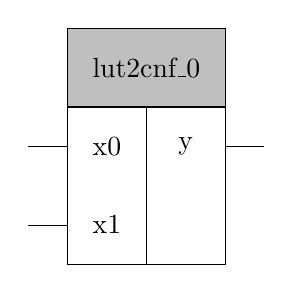
\begin{tikzpicture}

% instance name section
\filldraw[fill=lightgray] (0,2) rectangle (2,3);
\node (instancename) at (1,2.5) {lut2cnf\_0};

% input port section
\draw (0,0) rectangle (1, 2);
\node (portX0) at (0.5, 1.5) {x0};
\node (portX1) at (0.5, 0.5) {x1};
\draw (-0.5, 1.5) -- (0, 1.5);
\draw (-0.5, 0.5) -- (0, 0.5);


% output port section
\draw(1, 0) rectangle (2, 2);
\node (portY) at (1.5, 1.5) {y};
\draw (2, 1.5) -- (2.5, 1.5);

\end{tikzpicture} 
		\caption{An automatically generated component symbol}
		Based on listing \ref{code-minimal-descriptor}
		\label{fig-generated-symbol}
	\end{figure}
	
	Figure \ref{fig-generated-symbol} shows the subdivision of the symbol in three main areas.
	On the top, the instance name is centred, while the left side contains all input ports, and output ports are positioned to the right.
	The position of the port symbols is calculated during the creation of the circuit symbol and added to the component descriptor.
	It is not required to specify port positions in the descriptor file, as long as no custom symbol is used.
	
	\paragraph{User-Specified Circuit Symbols}
	Sometimes, it feels more convenient to the user to define their own symbol for certain component types, either because they are accustomed to them or because they want to convey additional information by visual means.
	This can be achieved by modifying the descriptor file.
	It is only required:
	
	\begin{itemize}	
		\item to add the property \texttt{symbolFile}, which specifies the location of the \gls{svg}-file containing the circuit symbol relative to the descriptor files location, and
		
		\item to extend the port descriptors by the positions, where to place the port symbols in the schematic.
		They are specified as a cartesian coordinates relative to the origin of the specified symbol file
	\end{itemize}
	
	An example can be found in listing \ref{code-modified-descriptor}.
	Note that the unaffected sections \texttt{name}, \texttt{configBits} and \texttt{functions} have been shortened to focus on the relevant changes.
	
	\includecode[json]{sources/descriptor-modified.json}{A descriptor file with a custom circuit symbol}{code-modified-descriptor}	
	
\subsection{Methods for Specifying Functional Behaviour}
	\label{sec-functional-behaviour-spec}
	
	While working with \emph{q2d}, it may become necessary to specify formulae.
	Two common examples are the \glspl{pcbd} contained in component descriptors and the specification of the target behaviour.
	Both cases shall be examined further in the paragraphs below.	
	
	\paragraph{General Considerations}
		Any formulae are specified in propositional logic.
		From a user's perspective, all behaviour is input as a list of strings.
		The elements of this list are treated as if they were conjuncted.
		Depending on the context, the set of valid variables may vary.
		
		For the convenience of users, different notations for logical operators are allowed.
		It is possible to either use symbols or mnemonics.\footnote{
			The recognition of mnemonics is case-sensitive.
			This might change in the future.
		}
		They are listed in table \ref{tab-logical-operators}.
		
		\begin{table}
			\centering
			\begin{tabular}{|r|crclc|}
				\hline
				Operator		& Type	& \multicolumn{3}{c}{Symbols}			& Mnemonic		\\
				\hline
				Negation		& prefix	& \textasciitilde \-	& \emph{or}	& !	& \texttt{not}	\\
				Conjunction	& infix	& \&	 				& \emph{or} 	& *	& \texttt{and}	\\
				Disjunction	& infix	& $|$ 				& \emph{or} 	& +	& \texttt{or}	\\
				Negated Conjunction	& infix & \multicolumn{3}{c}{\emph{(none)}}	& \texttt{nand}	\\
				Negated Disjunction	& infix	& \multicolumn{3}{c}{\emph{(none)}}	& \texttt{nor}	\\
				Exclusive Disjunction	&infix	& \multicolumn{3}{c}{\^}	& \texttt{xor}	\\
				Negated Exclusive Disjunction	&infix	& \multicolumn{3}{c}{\emph{(none)}}	& \texttt{xnor}	\\
				\hline
			\end{tabular}
			\caption{Overview of Logical Operator Notations in \emph{q2d}}
			\label{tab-logical-operators}
		\end{table}			
	
	\paragraph{Notation Styles}
		It is possible to use a clause notation like
		\begin{equation}
			\begin{aligned}
			&[ x, !y, z ] \\
			&[ x, y, !z ]
			\end{aligned}
		\label{eqn-styles-cnf}
		\end{equation}
		In this case, square brackets are used to delimit the clause, while commas separate the terms from each other.
		Unlike strict \gls{cnf}, a clause may not only contain literals but whole boolean expressions.
		
		The clauses of equation \ref{eqn-styles-cnf} could be re-written into a single expression:
		\begin{equation}
			(x\,|\,!y\,|\,z) \& (x\,|\,y\,|\,!z)
		\end{equation}
		
		As another often convenient alternative one might specify a boolean equation:
		\begin{equation}
			a = (b\ \text{or}\ c)\ \text{and}\ \text{not}\ d
		\label{eqn-styles-equation}
		\end{equation}
		Any non-\gls{cnf} style allows the usage of the equality operator and parenthesis to express precedence.
		The example in equation \ref{eqn-styles-equation} may be transcribed as
		\begin{equation}
			a \Leftrightarrow \left( b \vee c \right) \wedge \left(\neg d \right)
		\end{equation}
		
		It was shown in equation \ref{eqn-resolve-equivalence} how the equivalence can be resolved.
		The clause notation is mainly found in descriptor files.
		Each function represents one clause and all functions combined create a complete \gls{cnf} specification due to the line conjunction behaviour mentioned before.
		For most humans though, it feels more intuitive to specify boolean formulae, which results in this version being frequently used for specifying target formulae.
		
	
	\paragraph{\Glspl{cbd} in Descriptor Files}
		When creating component descriptors, it is often necessary to express the behaviour of a component.
		For that purpose, the descriptor files contain a \emph{functions}-section. 
		Within these functions, there is only a limited set of valid variables:
		\begin{description}
			\item[ports] represented by their respective names as provided in the \emph{ports}-section, as shown in listing \ref{code-minimal-descriptor}, lines 3 to 8.
			\item[configuration bits] that are named by taking the respective bit group name, adding an underscore and a corresponding incremental 0-based index number.
		\end{description}
		
	\paragraph{Target Formulae for SAT-solving}
		A target formula requires a module to be applied on.
		Any module interface name is a valid variable within the target function.\footnote{
			All releases of the application, up to the time of writing, accept	the full identifier of any component port as a variable as well.
			This behaviour seems to have no benefits regarding productive use so far, but proved useful for debugging. 
		}

\chapter{Implementation Details}
	\label{sec-chapter-implementation}
	
	In this section, implementation details of the application will be discussed.
Since the actual source files contain several thousands line of code, as well as dozens of classes and methods, it is not viable to explain everything in detail.
Therefore, several simplifications have been made in the following, to maintain the focus on the presented features.

\begin{itemize}
	\item All classes and methods that belong to the tool's implementation always reside in the super-namespace \texttt{q2d}, even if not explicitly stated.
	
	\item Classes that originate from \gls{qt} are not explicitly marked as such.
	They still can be easily spotted since it is a convention within the framework that all class names are prefixed with an uppercase letter \emph{Q}.
	\item The presentation has been reduced to focus on the main structure.
	For this reason, accessors, attributes and methods used for bookkeeping or as helpers have been omitted unless they are in some way important for explanatory reasons.
	
	\item Code elements, that were already considered deprecated at the time of writing, also have been left out.
\end{itemize}

Any description given here naturally can only reflect the application's state at a certain point in time.
To obtain further information on implementation details, it is strongly recommended to check out the project repository from \gls{github}.\footnote{
	\url{github.com/fer-rum/q2d}
}
In addition to the documentation delivered with the source code, a wiki is available at this site to help answering questions the user might have.\footnote{
	Should the wiki not be able to provide a satisfying answer, an issue should be opened, which will cause the developers to expand the wiki to cover the posed question as well. 
}

\Gls{uml} diagrams have been added to this document to aid understanding.
They can be found in appendix~\ref{sec-appendix-uml}
	\section{Classes Involved in the Component Meta-Model}
	\label{sec-metamodel}
	The \emph{component meta-model} has been established in section \ref{sec-model-design}.
	Its implementation can be found in the \texttt{q2d::metamodel}-namespace.
	Each part of the class hierarchy inherits from \gls{qt}'s \texttt{QObject} and \texttt{QStandardtem}.
	This is mainly to make use of the model-view capabilities delivered by the framework and ease the representation of the hierarchy in the \gls{ui} considerably.

	\paragraph{Overview over Elements}
	Everything in the meta-model is considered an \emph{element} of the model.
	Elements possess a \emph{type}, a \emph{name}, and may have another element as \emph{parent}.
	The type may be one of those listed in the \emph{element type} enumeration.
	Setting the name is achieved by using the \texttt{QStandardItem} constructor, while the parent relationship is inherited from \texttt{QObject}, narrowing down the type.
	
	The treelike structure of the meta-model is created by the subclass of \emph{hierarchy elements}.
	Additionally to their name, they also have a \emph{hierarchy name}, which serves as unique identifier, since it includes the names of all parent elements in addition to the elements own name.
	The principle is similar to absolute path names used in \glspl{os}.\footnote{
		Later during the implementation, a comparable naming and identification system for component instances had been introduced.
		Since both systems are very alike it is possible, that they will be merged eventually.
		The \texttt{Identifiable} class is discussed in section \ref{sec-documentEntry}.
	}
	Further, hierarchy elements are restricted to only accept \emph{categories} as parents.
	The intention is, to avoid that component types contain other component types, or even themselves.
	A nesting of categories on the other side poses no problem.
	
	Since \emph{component types} are the focus of the meta-model, it is obvious, to have a subclass for \emph{component elements}, from which component types can then be composed.
	Contrary to their superclass, these are restricted to component types as parent elements. 
	
	\paragraph{Categories}
	To keep an overview over many component types, categories have been introduced.
	They may contain an arbitrary set of \emph{component descriptors} or other sub-categories.
	In the \gls{ui} representation, categories can be expanded and collapsed by the user to help maintaining an overview or finding certain elements.
	
	\paragraph{Component Descriptors}
	As motivated in section \ref{sec-model-design}, an abstraction into component types was desired.
	This task is fulfilled by the \texttt{ComponentDescriptor}-class.
	It acts the as parent element for everything that is needed to describe a component type's behaviour and available ports.
	Further, information about the visual representation of a component are stored.
	Instances of this class are derived from the user definitions as discussed in section \ref{sec-user-defined-components}.
	
	\paragraph{Port-, Function-, and Configuration Bit Group Descriptors}
	When creating a component type, sub-descriptors are required.
	These are also provided by the descriptor files.
	Connection facilities are covered by \emph{port descriptors}, specifying their direction and the position relative to the component symbols origin.
	
	A \gls{pcbd}, as established in sections \ref{sec-definitions} and \ref{sec-functional-behaviour-spec}, is represented by a \emph{function descriptor}.\footnote{
		Careful readers might note that \glspl{pcbd} are, strictly speaking, no functions at all.
		This became clear during the work on the assignment, the name stuck however.
	}
	The fact that \glspl{pcbd} are given as strings, is reflected in the rather simple constructor.

	Additionally, component types may include \emph{configuration bit groups}.
	These are given by a name and a number of members, and upon adding them to a \texttt{ComponentDescriptor}-instance, will be expanded into a set of separate \emph{configuration bits}.
	
	\paragraph{Configuration Bit Descriptors}
	Contrary to the other parts of a component descriptor, these are not explicitly described in the respective file but are created by \emph{q2d} to have representative elements for each configuration bit in the component.
	This becomes useful when generating the solution to the \gls{qbf} problem.
	
	
	
	\section{The Document Entry Class and its Factory}
	\label{sec-documentEntry}
	Section  \ref{sec-basic-interaction} established the management of data in \emph{documents}.
	Since each of these documents describes a circuit as a whole, it is obvious that a data structure must exist, that can represent the elements of which the circuit is constructed.
	This is achieved by introducing \emph{document entries}.
	A \gls{uml}-representation of the classes discussed in the following is given in figure \ref{fig-class-diagram-documentEntry}.	
	
	\paragraph{The Environment of Document Entries}
	Any document entry needs to be associated with exactly one \emph{document}, which in turn might contain an arbitrary number of entries.
	Amongst each other, entries that belong to the same document can form hierarchies.
	Like all classes in the application, that might be involved in such a parent-child relationship, the \texttt{DocumentEntry} class inherits from \texttt{QObject}.
	As an additional feature, this also provides access to \gls{qt}s \emph{signal-slot} syntax, reducing the effort of implementing the communication between class instances notably.
	Internally, the application is split into a \emph{model}, holding the circuits structure and a \emph{schematic} representation, used by the \gls{ui}.
	A document entry acts as a controller to the two, subjecting them to changes depending on the operations issued by the user.
	It therefore is also called a \emph{related entry}.
	Since depending on the underlying model- and schematic elements, different interactions are possible, each document entry possesses a type which indicates what kind of elements it represents.\footnote{
	Subclassing \texttt{DocumentEntry} also would have been a viable	option.
	The projected gains however did not accommodate for the required efforts during the initial design.
	As always, this might change in the future, should the need arise.
	}
	This subdivision is discussed further in section \ref{sec-model-view}.
	Document entries are aware of the overall \emph{model} and \emph{schematic} indirectly through their parent document, and offer accessors to them for convenience reasons. 

	
	\paragraph{The \texttt{Identifiable} Helper Class}
	From the hierarchical structure of documents and their entries, the need to identify them by a name arose.
	For this reason, a helper class was developed, providing an abstraction for classes that require their instances to be recognized by a unique token.
	Upon the generation of such an identifiable object, it is only required to provide a \emph{local name}, and an optional parent object.
	Should the latter not be given, the current object may serve as root of a new hierarchy.
	A so-called \emph{full ID} consists of a local ID prepended with the name of each parent up to the hierarchies root.
	
	To aid with conceptualization, it is helpful to think of a file system, where the local name is only the file or folder name per\-se and the full ID can be compared to an absolute path.
	
	A useful result of this approach is the possibility to query any given document for an entries full ID and obtain the corresponding object, if there is one.
	Also, the \texttt{Identifiable} class creates a central point of validation for all IDs used throughout the application.	
	
	\paragraph{The Document Entry Factory}
	Instantiating document entries requires a lot of secondary tasks, such as ID validation, construction of model- and schematic elements, bookkeeping.
	To ease the effort and reduce the likelihood of errors, a factory class has been introduced, which takes care of all the matters that are associated with instantiating a \texttt{DocumentEntry}.
	For this purpose, a set of functions is offered to create entries for each possible type.
	Since ports are always sub-entries to some component or module interface\footnote{
		Module interfaces have been introduced in section \ref{sec-visualization-aspects}.	
	}
	, they are not instanced independently and therefore the corresponding helper function was omitted here.
	The default value for any of the IDs is invalid, triggering the factory to generate a valid one as a replacement.
	Since the user usually does not want to bother with naming everything in advance, this behaviour was deemed desirable.
	
		
	
	
	\section{Model and View}
		\label{sec-model-view}
		
		A lesson learned from the analysis of \gls{qucs} in the early stage of development was, that the separation of the internally kept model from the \gls{ui} representation is imperative to maintainability and extendibility of an application.
For this reason, \emph{q2d} keeps the structure of the designed circuit independent of the visualization as a schematic. 

To allow changes on the one side to be reflected on the other, document entries have been introduced in section \ref{sec-documentEntry}.

Since \gls{qt} introduces a model-view relationship within its \gls{ui} classes as well, in the following the term \emph{model} will always refer to the circuit representation, if not explicitly stated otherwise.

Due to the amount of classes involved in the discussed area and their fine distinctions, in the following, a class-centred description will be given instead of a full-text presentation.
This also is intended to help the reader find specific information more quickly.

A \gls{uml} representation of the described model is given in figure \ref{fig-class-diagram-model}.
		\subsection{The Model Element Hierarchy}
	\label{sec-model-hierarchy}

\begin{description}
	\item[Models] belong exclusively to one document each and complementary, each document has exactly one model. 
	Both objects in this relationship are aware of each other.
	Viewed hierarchically, the model is subordinate to the document.
	This is reflected by employing \texttt{QObject}s parent property.
	It also allows to take advantage of the behaviour that deleting the parent object will trigger the deletion of all children as well, thus avoiding memory leaks.
	Models consist of a set of \emph{model elements} that may be added via specialized methods. 
	
	\item[Model Elements] are first mentioned in section \ref{sec-documentEntry}, where each \texttt{DocumentEntry} instance holds one model element, which in turn considers the entry \emph{related}.
	Such model element has exactly one model as a hierarchical parent, which is just the model that belongs to the document the related document entry is part of.
	For convenience reasons, model elements offer access to their related entries ID accessors.
	
	It is required, for solving the \gls{qbf} problem, that each model element can yield information about the contained \emph{configuration}, \emph{input} and \emph{node} variables as well as any \glspl{pcbd}\footnote{
		Again, for historical reasons, the getter is called \texttt{functions()}, even though \glspl{pcbd} are no functions at all.	
	}.
	As a default implementation, the returned lists are empty, but sub-classes will override this behaviour, if required.
	Lastly, a \emph{property map} may be requested, that contains information about the internal state of the model element.
	This is used for debug purposes as well as for the generation of tool tips by schematic representations.
	
	\item[Interfacing Model Elements] form a specialized sub-class which offer the additional capability of managing ports.
	When queried for node variables, they query each of their ports and yield a collection of the results.
	
	\item[Components] are created by the use of a \texttt{ComponentDescriptor}, which was introduced in section \ref{sec-metamodel}.
	Multiple components may share the same descriptor, effectively making them instances of the same type of component.
	In addition to the inherited node variable getter, they can also provide configuration variables and \glspl{cbd} as defined by their descriptor.
	
	\item[Module Interfaces] are \texttt{InterfacingME}s, that have exactly one port and a direction determining the orientation of the data flow as viewed from the \emph{outside} of the module.
	As a result, the directions given in the module interface and its port are opposites of each other.
	
	\item[Nodes] are any elements that are driven by one signal source and may distribute this signal unaltered.\footnote{
		Since in some contexts, the terms \emph{driver} and \emph{driven} may be used with different semantics, it is in the following also feasible to read \emph{data source} and \emph{data sink} instead, respectively.	
	}
	Currently, the only actual implementation of nodes are ports used for connecting interfacing model elements with each other.
	Technically, conductors should be considered nodes as well but, at the time of writing, no need has arisen to implement it that way.\footnote{
		The underlying reason is, that conductors only represent a one-to-one connection, which is fairly trivial.
		Should these simple conductors be replaced by wire nets as done in other tools, such a net could be validly considered a node and be consequently implemented as such.	
	}
	
	\item[Ports] additionally possess a \emph{direction} that specifies whether data passing the port flows into the interfaced element or out of it.
	They further provide a custom property map, containing additional information about their connection state.

	\item[Component ports] facilitate the data transfer into and out of components.
	If queried, they return a node variable, representing themselves.
	
	\item[Module ports] are used exclusively by module interfaces.
	If the instance's \texttt{direction} is \texttt{OUT}, the associated module interface has an \texttt{IN} direction.
	Therefore, the port is to be represented by an input variable.
	Otherwise, it will yield an appropriate node variable.
	
	\item[Conductors] are intended to connect interfacing elements with each other.
	Precisely speaking, they transfer data from one node to another.
	For this reason, they distinguish a sender and a receiver node.
	While from the senders view, the conductor acts as a driven element, for the receiver, it becomes a driver.
	While each conductor in the implementation only connects one sender to one receiver, many other tools instead abstract at the level of whole wiring nets.\footnote{
		It was discussed following these examples but no such changes were made up to the time of writing since it was found not realistic to implement the required changes within the given time frame. Also, the nomenclature of \emph{nodes} would have to change for consistency reasons.
	}
	Each conductor yields its sender and receiver as node variables and a $\sigma$-term as defined in equation \ref{eqn-define-sigma}.
\end{description}
		\subsection{The Schematics Element Hierarchy}

For implementing the \gls{ui}, heavy use of facilities offered by \gls{qt} has been made.
This especially refers to the graphics framework, which already provides most of the base classes necessary to implement graphical representations and define user interaction.
Due to the size of this framework, it cannot be explained here in detail.
The reader might want to consult the \gls{qt} reference %TODO cite qt doc
in parallel for detailed information on these classes and their interaction.
When classes are derived from the framework, they often need to override specific functions to achieve custom behaviour.
These overrides have been omitted in figure \ref{fig-class-diagram-schematic} to avoid cluttering the diagram.

\begin{description}

	\item[Schematic] is a specialization of a \texttt{QGraphicsScene}. 
	It acts as container for elements to be displayed to the user.
	Each schematic belongs to exactly one document and visually represents the documents model.
	In turn, each document holds exactly one schematic, while its entries offer a convenience getter to the latter.
	
	\item[Schematic elements] are specializations of \texttt{QGraphicObject}.
	A hierarchical connection between the schematic and its elements is constructed via the \emph{scene-item relationship}, already provided by \gls{qt}'s graphics framework.
	A schematic element might have an arbitrary number of sub-items, called \emph{actuals}.
	These act as building blocks for the graphics displayed to the user.
	This hierarchical approach ensures that modifications like moving an element on the schematic view, will be applied to the actuals as well, while offering also flexibility to modify only selected sub-items.
	Further, the \texttt{scene()} getter has been overridden, to return the schematic, instead of a generic \texttt{QGraphicsScene}.
	A schematic element may provide \texttt{additionalJson()} and a \texttt{specificType()} that are used for serialization purposes.
	
	\item[Parent Schematic Elements] are a specialization of schematic elements that has been introduced for type safety reasons.
	Again, the dependency between these elements and their hierarchical children already is given by means of the graphical framework.
	
	\item[Component Graphics Items] represent components on the schematic.
	They are associated with the appropriate component descriptors, similar to their \texttt{Component} counterparts in the model as described in section \ref{sec-model-hierarchy}.
	The hierarchy name of the descriptor will be used as the specific type in the \gls{json} files to allow a re-creation of the component graphics item, even if the descriptor should change between saving and loading.
	
	\item[Module Interface Graphics Items] visually represent the connections of the circuit to the outside world.
	The concept has been introduced in section \ref{sec-visualization-aspects}.
	As stated there, module interfaces feature a \texttt{direction}, which specifies, if data flows into or out of the interfaced circuit.
	
	\item[Port Graphic Items] are implementations of the concepts regarding port visualization presented in section \ref{sec-visualization-aspects}.
	Unlike their counterparts in the model, no specializations had to be made since their representation is agnostic of the element they are interfacing.
	Since connecting ports with each other is done by dragging a connection from an output port and dropping onto an input port, a set of event handling functions had to be customized to allow this interaction.
	For the same purpose a distinct \texttt{wireDrawingMode} had to be introduced.
	
	\item[Wire Graphics Items] visualize a data-transmitting connection from one port to another.
	Each wire has a data width of exactly one bit.\footnote{
		Multiple bit wide connections or bus systems were considered very work intensive and were scheduled for a later release.
		They can alternatively be emulated by appropriate components, so users do not have to forgo this kind of feature completely.
	}
	Wires will be routed automatically.
	For this purpose, they are internally split into \texttt{WireGraphicsLineItem}s, which will be created in the process.
	The currently implemented routing algorithms are not very sophisticated yet, but already suffice for a huge amount of circuit designs.\footnote{
		Especially referring to designs without loop-backs.	
	}
	If the start or end port is moved, the wire will be automatically re-routed.
	When hovered by the mouse, all elements of a wire will highlight to help the user tracking its path.
	For data persistence, the wire graphics items offer a specialized additional \gls{json} object that contains the full identifiers of the start and end port.
	Upon loading, the wire is routed again, so that any new algorithms available for this purpose are applied without user intervention.

\end{description}

		\section{The Quantor Interface}
	\label{sec-quantor-interface}
	The computation of the \gls{qbf} solution using \gls{quantor} as outlined in section \ref{sec-solving-qbf} is very straight-forward.
	\Gls{quantor} itself is written in \emph{C}, so bridging classes to \emph{C++} were created.
	Further, it is requited to build the contexts and transform them to \gls{cnf}.
	At this point, the \gls{qbf} solver can take over.
	Upon completion, it returns a structure representing the result, which again will be wrapped into a \emph{C++} class.
	
	\paragraph{The Solving Process}
	The whole \gls{qbf} solving process is controlled by the \texttt{QuantorInterface}.
	It inherits \texttt{QObject} since this enables it to use \gls{qt}'s \emph{signal and slot system}. %TODO cite
	This method of program-internal communication will trigger the solving process via the \texttt{slot\_solveProblem()}.\footnote{
		A lot of other classes discussed earlier use this mechanism for communication as well.
		It has not been explicitly mentioned so far, to keep things straightforward.
	}
	
	If posed with a problem, the target document will be queried for the model, from which the contexts can be build.
	Once available, these are fed into the \texttt{Quantorizer}, which in turn transforms them in a form that \gls{quantor} will accept as an input and trigger the actual evaluation of the \gls{qbf}.
	
	Upon completion, the solver will deliver a verdict, which might be either \emph{satisfiable}, \emph{not satisfiable}, \emph{out of time} or \emph{out of memory}.
	In the first case, it will also return a set of integer numbers, representing the solution found.
	The result object is interpreted by the \texttt{QuantorInterface} which will then present the verdict as a string and, if applicable, a mapping from the full IDs of configuration bits to their boolean value assignments that solve the problem.
	The found answer is propagated by emitting the \texttt{signal\_hasSolution()}

	\paragraph{Variable Representation in Quantor}
	Internally, \gls{quantor} represents each variable by an integer number greater than zero.
	When using literals in clauses, the number of the variable is employed unaltered to represent a positive literal or inverted to represent a negative literal.
	
	\paragraph{Context Creation in Detail}
	It is a responsibility of the context creation process to provide a consistent mapping of the full IDs of variables yielded by model elements to their numerical representations to be used by \gls{quantor}.
	One context will be created for each interfacing model element, implementing the theoretical approach of equation \ref{eqn-define-box-epsilon}.
	Additionally, there is a \emph{global context}, in accordance with equation \ref{eqn-define-box}.
	Unlike the theoretical approach, the actual implementation does not merge all sets of variables and terms but rather keeps all model element contexts as children of the global context.
	This allows the re-use of already created \texttt{QIContext} instances.
	The resulting lookup overhead due to traversing an additional hierarchy level for variables was found to have a negligible impact on the time of problem solving.
	A further motivation for this approach was the specification of \glspl{cbd} in descriptor files.
	These use only local names since it is not known, before instantiating a component, what its name will be and, in turn, what the full IDs of the used variables will be.
	Re-naming them appropriately in each of the \glspl{pcbd} after component instantiation did not appear to offer any considerable benefits for the effort.
	For the proper assignment of variables to their numeric counterparts, a context must be aware of the range of values it can use for the mapping.
	Such a value is also called an \emph{index}.
	Since contexts are not created in parallel but one after another, this can be easily achieved by passing the lowest index to be used when instantiating a \texttt{QIContext} instance.
	It will then collect all variables yielded by the abstracted model element.
	Upon encountering a new variable, a lookup will be made to see if it has already occurred in another context.
	This might for example be the case for node variables which occur in \glspl{pcbd} as well as $\sigma$-formulae.
	Should this be the case, the variable's already known index will be adopted.
	Otherwise, the current index will be incremented and mapped to this variable.
	Once all variables are processed this way, the current index is the highest index used by this context and will be passed on to the next context to be used as its lower index bound.
	In the next step, all connections within the model elements are evaluated and $\sigma^*$ as defined in equation \ref{eqn-define-sigma-star} is introduced to the problem description.
	Lastly, the context also collects all \glspl{pcbd} contained in the model element, or, in the case of the global context, the target formula.
	
	\paragraph{The Quantorizer}
	To transform the information gathered during context creation into a form which is suitable as input for \gls{quantor}, the \texttt{Quantorizer} will parse all \glspl{cbd} as well as the target formula.\footnote{
		The \emph{quantorizer} essentially is a parser, created by the parser generator \emph{wisent}\cite{wisent}.	
	}
	If any given boolean term cannot be parsed properly due to input errors or corrupted descriptor files, a \texttt{ParseException} will be thrown and the solving process will be aborted, reporting an error.\footnote{
		Depending on the version of \emph{q2d} used, error reporting might be facilitated by printing to \texttt{stderr}.
		\Gls{ui} support for error messages was introduced relatively late in the development process.
		It can be useful to launch the application from the console to not miss any messages.	
	}
	Otherwise, the variables contained in the term or function will be looked up and their indices used to create clauses, to be added to \gls{quantor}'s description of the problem.
	Once done, the solver can proceed to work on the problem.
	Its result will be returned to the \texttt{QuantorInterface}.
	
	\paragraph{Interpreting the Result}
	The result is emitted in two parts by the \texttt{Quantorizer}.
	A \texttt{Result}-object is returned from the call to \texttt{solve()}, and the vector given as a parameter will be filled with the literal assignments of the solution.
	While the returned object can be cast to a string to obtain a textual representation, the vectors content has to be resolved back to full IDs.
	The sign of an element of the vector expresses if this certain variable should be configured to be either true or false.
	In doing so, a human-readable interpretation of the solution can be obtained and will be presented to the user in tabular form.
	
\chapter{An Example Workflow}

	\section{The Task}
	\label{sec-workflow-task}
	To illustrate how \emph{q2d} can be used productively, consider the following workflow example.
	For this purpose, a \gls{clb} as it is used in \textsc{Xilinx Virtex 5} \glspl{fpga} is to be modelled.
	A circuit diagram of the part in question is given in figure \ref{fig-clb-detail}.
	More information regarding the actual architecture can be found in the official manual.\footnote{
		Available at \url{www.xilinx.com/support/documentation/user_guides/ug190.pdf}
	}\cite{virtex5}
	Further, the configuration required to realize a \emph{full adder} with this model shall be computed.

	\begin{figure}[p]
	\centering
		\resizebox{0.9\textwidth}{!}{
		
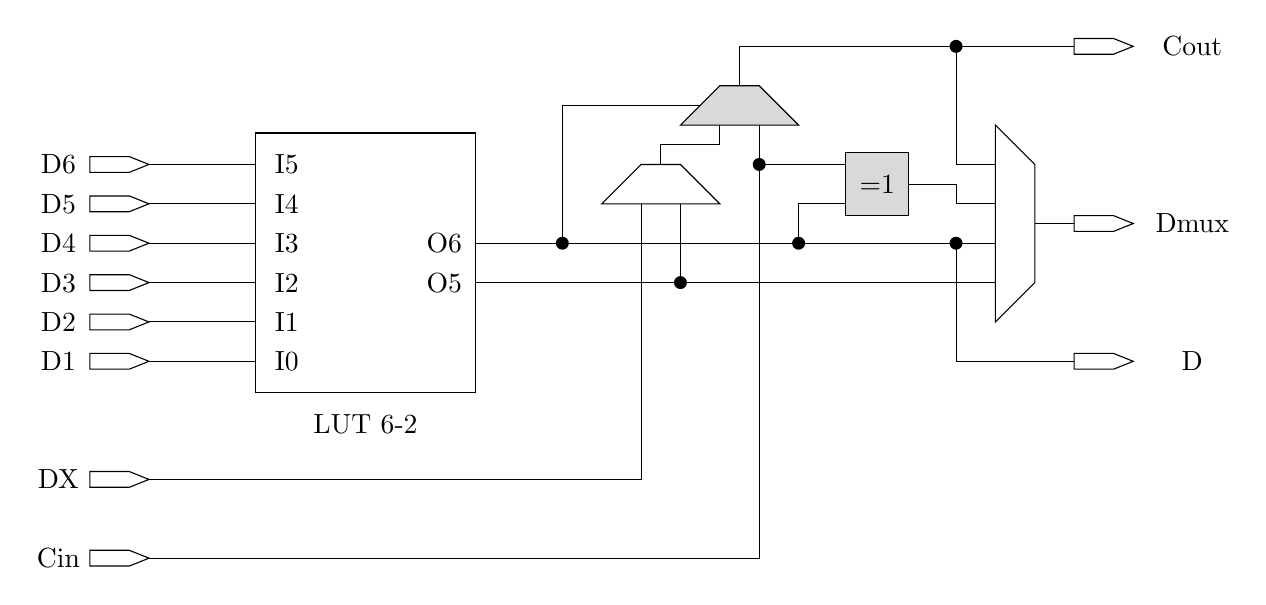
\begin{tikzpicture}

% inputs
\draw (0mm, -1mm) -- (5mm, -1mm) -- (7.5mm, 0mm) -- (5mm, 1mm) -- (0mm, 1mm) -- cycle;
\draw (0mm, 4mm) -- (5mm, 4mm) -- (7.5mm, 5mm) -- (5mm, 6mm) -- (0mm, 6mm) -- cycle;
\draw (0mm, 9mm) -- (5mm, 9mm) -- (7.5mm, 10mm) -- (5mm, 11mm) -- (0mm, 11mm) -- cycle;
\draw (0mm, 14mm) -- (5mm, 14mm) -- (7.5mm, 15mm) -- (5mm, 16mm) -- (0mm, 16mm) -- cycle;
\draw (0mm, 19mm) -- (5mm, 19mm) -- (7.5mm, 20mm) -- (5mm, 21mm) -- (0mm, 21mm) -- cycle;
\draw (0mm, 24mm) -- (5mm, 24mm) -- (7.5mm, 25mm) -- (5mm, 26mm) -- (0mm, 26mm) -- cycle;

\draw (-4mm, 0mm) node {D1};
\draw (-4mm, 5mm) node {D2};
\draw (-4mm, 10mm) node {D3};
\draw (-4mm, 15mm) node {D4};
\draw (-4mm, 20mm) node {D5};
\draw (-4mm, 25mm) node {D6};

% lut
\draw (25mm, 0mm) node {I0};
\draw (25mm, 5mm) node {I1};
\draw (25mm, 10mm) node {I2};
\draw (25mm, 15mm) node {I3};
\draw (25mm, 20mm) node {I4};
\draw (25mm, 25mm) node {I5};

\draw (45mm, 10mm) node {O5};
\draw (45mm, 15mm) node {O6};
\draw(35mm, -8mm) node{LUT 6-2};

\draw(21mm, -4mm) rectangle (49mm, 29mm);

% dx
\draw (0mm, -16mm) -- (5mm, -16mm) -- (7.5mm, -15mm) -- (5mm, -14mm) -- (0mm, -14mm) -- cycle;
\draw (-4mm, -15mm) node {DX};

% cin
\draw (0mm, -26mm) -- (5mm, -26mm) -- (7.5mm, -25mm) -- (5mm, -24mm) -- (0mm, -24mm) -- cycle;
\draw (-4mm, -25mm) node {Cin};

% mux
\draw[fill=gray!30!white](75mm, 30mm) -- (90mm, 30mm) -- (85mm, 35mm) -- (80mm, 35mm) -- cycle;

% cmux
\draw(65mm, 20mm) -- (80mm, 20mm) -- (75mm, 25mm) -- (70mm, 25mm) -- cycle;

% xor
\draw[fill=gray!30!white](96mm, 18.5mm) rectangle (104mm, 26.5mm);
\draw(100mm, 22.5mm) node{=1};

% cmux-d
\draw(115mm, 5mm) -- (120mm, 10mm) -- (120mm, 25mm) -- (115mm, 30mm) -- cycle;

%cout
\draw (125mm, 39mm) -- (130mm, 39mm) -- (132.5mm, 40mm) -- (130mm, 41mm) -- (125mm, 41mm) -- cycle;
\draw (140mm, 40mm) node {Cout};

%dmux
\draw (125mm, 16.5mm) -- (130mm, 16.5mm) -- (132.5mm, 17.5mm) -- (130mm, 18.5mm) -- (125mm, 18.5mm) -- cycle;
\draw (140mm, 17.5mm) node {Dmux};

%d
\draw (125mm, -1mm) -- (130mm, -1mm) -- (132.5mm, 0mm) -- (130mm, 1mm) -- (125mm, 1mm) -- cycle;
\draw (140mm, 0mm) node {D};

% wiring
	% inputs -> lut
\draw(7.5mm, 0mm) -- (21mm, 0mm);
\draw(7.5mm, 5mm) -- (21mm, 5mm);
\draw(7.5mm, 10mm) -- (21mm, 10mm);
\draw(7.5mm, 15mm) -- (21mm, 15mm);
\draw(7.5mm, 20mm) -- (21mm, 20mm);
\draw(7.5mm, 25mm) -- (21mm, 25mm);
	% O5 ->cmux
\draw[fill] (75mm, 10mm) circle (.75mm);
\draw(49mm, 10mm) -- (75mm, 10mm) -- (75mm, 20mm);
	% DX ->cmux
\draw(7.5mm, -15mm) -- (70mm, -15mm) -- (70mm, 20mm);
	% cmux -> mux
\draw(72.5mm, 25mm) -- (72.5mm, 27.5mm) -- (80mm, 27.5mm) -- (80mm, 30mm);
	% cim -> mux
\draw(7.5mm, -25mm) -- (85mm, -25mm) -- (85mm, 30mm);
	% O6 -> mux
\draw[fill](60mm, 15mm) circle (.75mm);
\draw(49mm, 15mm) -- (60mm, 15mm) -- (60mm, 32.5mm) -- (77.5mm, 32.5mm);
	% O6 -> xor
\draw[fill](90mm, 15mm) circle (.75mm);
\draw(60mm, 15mm) -- (90mm, 15mm) -- (90mm, 20mm) -- (96mm, 20mm);
	% Cin -> xor
\draw[fill](85mm, 25mm) circle (.75mm);
\draw(85mm, 25mm) -- (96mm, 25mm);
	% O5 -> cmux-d
\draw(75mm, 10mm) -- (115mm, 10mm);
	% O6 -> cmux-d
\draw(90mm, 15mm) -- (115mm, 15mm);
	% xor -> cmux-d
\draw(104mm, 22.5mm) -- (110mm, 22.5mm) -- (110mm, 20mm) -- (115mm, 20mm);
	% mux -> cout
\draw(82.5mm, 35mm) -- (82.5mm, 40mm) -- (125mm, 40mm);
	%mux ->cmux-d
\draw[fill](110mm, 40mm) circle (.75mm);
\draw(110mm, 40mm) -- (110mm, 25mm) -- (115mm, 25mm);
	%O6 -> d
\draw[fill](110mm, 15mm) circle (.75mm);
\draw(110mm, 15mm) -- (110mm, 0mm) -- (125mm, 0mm);
	% cmux-d ->dmux
\draw(120mm, 17.5mm) -- (125mm, 17.5mm);
\end{tikzpicture}
		}
		\caption{Circuit Diagram of a CLB Detail}
		White components are configurable.
		\label{fig-clb-detail}
	\end{figure}		

	\begin{figure}[p]
	\centering
		\resizebox{!}{0.4\textheight}{
		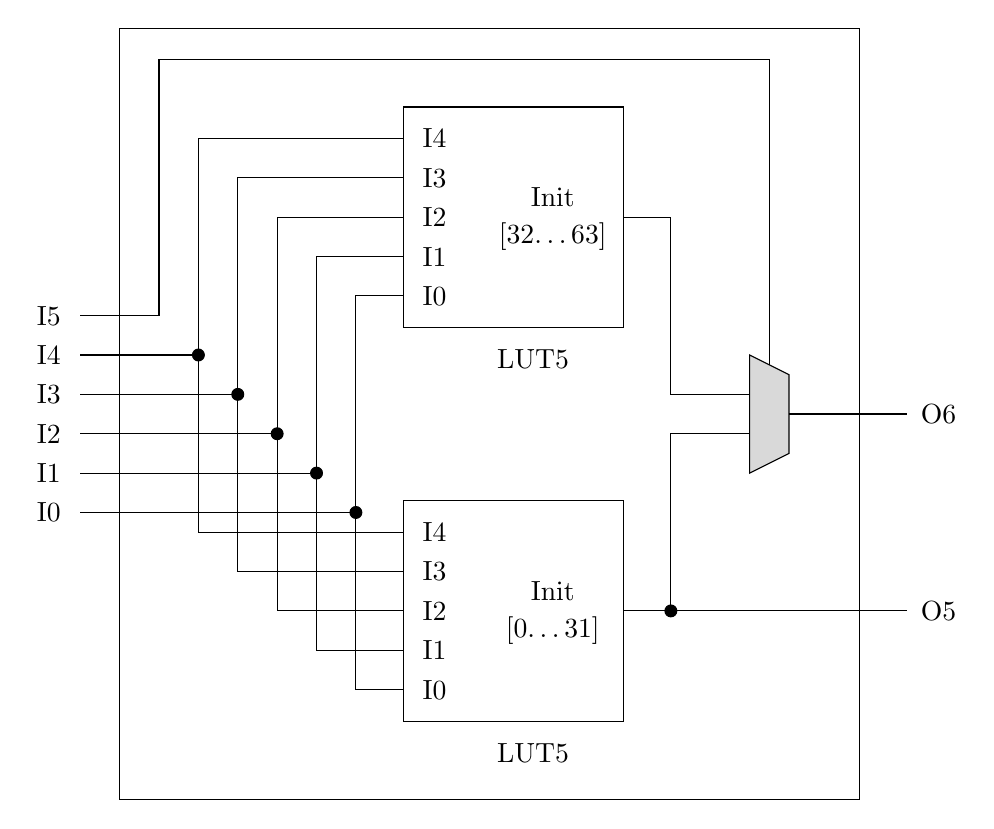
\begin{tikzpicture}

%lut6
\draw(-30mm, -49mm) rectangle (64mm, 49mm);
\draw(-39mm, 12.5mm) node{I5};
\draw(-39mm, 7.5mm) node{I4};
\draw(-39mm, 2.5mm) node{I3};
\draw(-39mm, -2.5mm) node{I2};
\draw(-39mm, -7.5mm) node{I1};
\draw(-39mm, -12.5mm) node{I0};

\draw(74mm, 0mm) node{O6};
\draw(74mm, -25mm) node{O5};

% lut1
\draw(6mm, 11mm) rectangle (34mm, 39mm);
\draw(10mm, 35mm) node{I4};
\draw(10mm, 30mm) node{I3};
\draw(10mm, 25mm) node{I2};
\draw(10mm, 20mm) node{I1};
\draw(10mm, 15mm) node{I0};

\draw(22.5mm, 7mm) node {LUT5};

\draw(25mm, 27.5mm) node {Init};
\draw(25mm, 22.5mm) node {[32\dots63]};

% lut2
\draw(6mm, -11mm) rectangle (34mm, -39mm);
\draw(10mm, -15mm) node{I4};
\draw(10mm, -20mm) node{I3};
\draw(10mm, -25mm) node{I2};
\draw(10mm, -30mm) node{I1};
\draw(10mm, -35mm) node{I0};

\draw(22.5mm, -43mm) node {LUT5};

\draw(25mm, -22.5mm) node {Init};
\draw(25mm, -27.5mm) node {[0\dots31]};

%cmux
\draw[fill=gray!30!white](50mm, 7.5mm) -- (50mm, -7.5mm) -- (55mm, -5mm) -- (55mm, 5mm) -- cycle;

%wiring
	%lut1 -> cmux
\draw(34mm, 25mm) -- (40mm, 25mm) -- (40mm, 2.5mm) -- (50mm, 2.5mm);
	%lut2 -> cmux
\draw(34mm, -25mm) -- (40mm, -25mm) -- (40mm, -2.5mm) -- (50mm, -2.5mm);

	%I0
\draw(-35mm, -12.5mm) -- (0mm, -12.5mm) -- (0mm, -35mm) -- (6mm, -35mm);
\draw[fill](0mm, -12.5mm) circle (0.75mm);
\draw(0mm, -12.5mm) -- (0mm, 15mm) --(6mm, 15mm);

	%I1
\draw(-35mm, -7.5mm) -- (-5mm, -7.5mm) -- (-5mm, -30mm) -- (6mm, -30mm);
\draw[fill](-5mm, -7.5mm) circle (0.75mm);
\draw(-5mm, -7.5mm) -- (-5mm, 20mm) --(6mm, 20mm);

	%I2
\draw(-35mm, -2.5mm) -- (-10mm, -2.5mm) -- (-10mm, -25mm) -- (6mm, -25mm);
\draw[fill](-10mm, -2.5mm) circle (0.75mm);
\draw(-10mm, -2.5mm) -- (-10mm, 25mm) --(6mm, 25mm);

	%I3
\draw(-35mm, 2.5mm) -- (-15mm, 2.5mm) -- (-15mm, -20mm) -- (6mm, -20mm);
\draw[fill](-15mm, 2.5mm) circle (0.75mm);
\draw(-15mm, -2.5mm) -- (-15mm, 30mm) --(6mm, 30mm);

	%I4
\draw(-35mm, 7.5mm) -- (-20mm, 7.5mm) -- (-20mm, -15mm) -- (6mm, -15mm);
\draw[fill](-20mm, 7.5mm) circle (0.75mm);
\draw(-20mm, 7.5mm) -- (-20mm, 35mm) --(6mm, 35mm);

	%I5
\draw(-35mm, 12.5mm) -- (-25mm, 12.5mm) -- (-25mm, 45mm) -- (52.5mm, 45mm) -- (52.5mm, 6.25mm);

	%O5
\draw(40mm, -25mm) -- (70mm, -25mm);
\draw[fill](40mm, -25mm) circle (0.75mm);

	%O6
\draw(55mm, 0mm) -- (70mm, 0mm);


\end{tikzpicture}


		}
		\caption{Circuit Diagram of Xilinx' LUT6-2 }
		\label{fig-lut}
	\end{figure}		

	\paragraph{How the Full Adder Will Work}
	When looking at the architecture, it is easy to see that it already provides a carry chain, which shall be used.
	The \texttt{Dmux} output will be used for the sum, which requires the \texttt{O6} port of the \gls{lut} to emit the propagate bit.
	It is notable, that the \texttt{D} output is directly attached to the respective wire, so it could be used as a proxy for the propagate bit.
	If the adder does not propagate, \texttt{Cout} will assume the value of the generate bit, which in turn has to be emitted by the port \texttt{O5}.
	Due to the \gls{lut}'s outputs having to assume different values, it is necessary to pin the input \texttt{D6} to \emph{true}, as can be inferred from the description given in section \ref{sec-xilinx-lut}.

\section{A Component Descriptor for Xilinx' LUT6-2}
	\label{sec-xilinx-lut}
	While multiplexers are not very complicated and very obvious to describe via a formula, the \gls{lut} deserves a closer look.
	A special variant, featuring six input ports, but only two output ports is employed here.
	Research of the actual components internals yields that it is composited from two 5-input \glspl{lut}.
	The sixth input determines whether both output ports will emit the same signal as determined by the lower \gls{lut} or different signals, originating from both \glspl{lut} independently. 
	This is depicted in figure \ref{fig-lut}, which also can be found in most of the official design guidelines\footnote{
		For example at \url{www.xilinx.com/support/documentation/sw_manuals/xilinx14_7/virtex5_hdl.pdf}	
	}\cite{hdl-guide}.
	Since no appropriate component descriptor for this type of \gls{lut} is commonly available yet, it has to be created from scratch.
	As outlined in section \ref{sec-user-defined-components}, this can be done even with a simple text editor.
	The resulting descriptor file is to be found in listing \ref{code-lut62-descriptor}.
	For overview reasons, the \texttt{functions} section has been shortened. 
	Since the clauses used as \glspl{pcbd} are very repetitive and systematic, users with some programming skills will most likely write a simple script to generate these lines.
	It can also be noted that there are different possible ways of describing the components behaviour correctly.
	
		\includecode[json]{sources/xi-lut6-2.json}{The Component Descriptor for Xilinx' LUT6\_2}{code-lut62-descriptor}

\section{Designing the Model}
	With all preparations made, it is simple to create the circuit within \emph{q2d}.
	In the following, a brief walk-through will be given.
	It will be assumed that a new project had been created and the current document is empty.
	
	\paragraph{Loading the Required Component Descriptors}
	Users, who start with a fresh copy of the application will most likely not yet have a set of components to choose from.
	They may either create the required component descriptors by themselves\footnote{
		Which is a great opportunity to get familiar with the component creation process.
	} or obtain such descriptors from separate sources\footnote{
		A collection of component descriptors can be found at \url{github.com/fer-rum/q2d-components}. 	
	}.
	The actual import can be done for each descriptor via the menu \menu{{Component Hierarchy} > {Add Component Type}}, which will then prompt for the descriptor file.
	 A component library feature to ease this task has been drafted at the time of writing but is still rudimentary.
	 
	\paragraph{Placing and Connecting Components}
	A Component will be placed by dragging the component descriptor from the component hierarchy onto the schematic.
	The schematic symbols can be dragged to another position 	at any time.
	Module interfaces can be created by clicking the appropriate button in the upper right corner of the document's tab and entering a unique name.
	Wire connections are created by dragging from the driving port and dropping at the driven port.
	 
	\paragraph{Pinning an Input to a Fixed Value}
	As noted in section \ref{sec-workflow-task}, it is required to make sure, that the input \texttt{D6} is always true.
	This can be achieved by connecting it to a component that always returns \emph{true}.
	Doing this directly in the target formulae is possible but a preferable alternative would be to create a component, which only has one output port \texttt{out} and for example

	\begin{verbatim}
		[out]
	\end{verbatim}
	
	as \gls{cbd}.
	Connecting an instance of this component type to \texttt{D6} will yield the desired results.
	This approach could be expanded by using a \gls{cmux}, which is fed by an \emph{always-true} component, an \emph{always-false} component and the actual module input\footnote{
		If desired, all this functionality could also be combined into one component.	
	}.
	Even more degrees of freedom can be obtained by connecting all module inputs to such a \gls{cmux}.
	Additionally, this allows to evaluate whether the signal in question needs to be pinned to a certain value or not.
	
\section{Computing the Desired Configuration}

	\paragraph{Applying the Target Formulae}
	The target formulae can be specified in a text input area near the upper border of the document's tab.
	Assuming that the module interfaces have been named according to figure \ref{fig-clb-detail}, a possible description of the desired full adder is
	
	\begin{verbatim}
	dmux = (d1 ^ d2) ^ cin
	cout = (d1 & d2) | ((d1 ^ d2) & cin)
	\end{verbatim}

	Here, the inputs \texttt{D1} and \texttt{D2} are used for the summands	, \texttt{Dmux} for the sum and \texttt{cin} and \texttt{cout} for the carry chain.
	Clicking the \menu{Check SAT} button will trigger the evaluation of the design with respect to the input target formulae.
	
	\paragraph{Interpreting the Output}
	A separate window will inform the user about the result of the solving process.
	At its top, the overall verdict will be printed in textual form\footnote{
		As mentioned before, earlier versions of the application did not report errors like malformed input to the \gls{ui} and rather printed a console message.
		Should no window for the solution appear, it is most likely, that additional information will be available there.	
	}.
	Further a configuration solving the \gls{sat} problem is presented in tabular form.
	Each configuration variable will be listed by its full ID together with the boolean value it has to assume to satisfy the target formulae.
	If a certain configuration bit is not included in the solution, its representing variable was eliminated during the solving process.
	Consequently the value assumed by this bit is not relevant for the \gls{sat} problem and the bit can be assigned an arbitrary value.
	
	\paragraph{Further Modifying the Document}
	When saved, the document is written out as a plain text \gls{json} file within the projects folder.
	This allowsits  easy modification outside of \emph{q2d}.
	By changing the documents file, users can achieve features not (yet) supported by the \gls{ui} at the time of writing.
	Examples are re-wiring, renaming or deleting model elements. 

\chapter{Summary and Outlook}	

	\section{Achieved Results}

	In this writing, the tool \emph{q2d}, its theoretical background and design were presented.
	
	\paragraph{Goal}
	The intention behind this work was to create an application that allows users to easily create a circuit design containing configurable components within a graphical \gls{ui} along with a specification of an intended behaviour.
	The tool evaluates whether this specification can be fulfilled by a component configuration and, if this is the case, also provides a configuration that solves the posed problem.
	It was established that this requires the solving of a \gls{qbf} problem and how the design can be described as such.
	
	\paragraph{Development and Design Decisions}
	Initially, it was intended to use \gls{qucs} as a code base and employ a pure \gls{sat} solver for evaluating the designed circuits.
	This approach turned out to be infeasible due to design issues and the state of \gls{qucs}' code at the time of writing.
	As a consequence, it was chosen to implement a new tool for the intended purpose.
	 From the experience made with the earlier attempt, several major design decisions were inferred:
	 
	 \begin{itemize}
	 
	 \item The application was developed using \gls{qt}.
	 	Retrospectively, the time invested in getting familiar with this framework seemed to be well invested due to the amount of work saved when dealing with common implementation tasks.
	 	
	 \item The \gls{qbf} solver \gls{quantor} has been employed instead of a pure \gls{sat} solver.
	 	This eradicated the need for intermediate file formats and streamlined the circuit evaluation process considerably.
	 
	 \item Components are not hard-coded.
	 	They instead reside in separate descriptor files, which are easy to write, read and adapt by users.
	 	
	 \item Component behaviour is described using boolean formulae or \gls{cnf}.
	 The same applies to the description of the intended functionality of the circuit.
	 Allowing different variations of specifying operators allows users to use the notation they prefer.
	 		 	
	 \item Automatically generated circuit symbols for components relief the users of providing such for each component type they design.
	 As a result, custom components can be developed even quicker.
	 
	 \end{itemize}
	
	\paragraph{Functionality and Appearance}
	Basic project and document management features are available and users are enabled to import and employ any component they have a descriptor file for.
	Several visualisation techniques have been employed to allow a faster orientation within the schematic design and improve the perception of relevant information.
	An emphasis has been put on the presentation of component ports.
	Additionally, \emph{details on demand} are available for all circuit elements.
	
	\paragraph{Implementation Details}
	The core classes of the application and their interaction with each other have been described.
	The focus mostly lies on their purpose and concepts.
	For the \texttt{QuantorInterface} the inner workings have been further elaborated . 
	It thereby was underlined how the theoretical approach was realized in the application.
	
	\paragraph{A Workflow Example}
	To demonstrate the usage of the tool, the schematic of a \emph{Xilinx Virtex 5} \gls{clb} has been reproduced, implementing the required custom components in the process.
	 It was shown that a \emph{full adder} could be implemented with such a \gls{clb}, by computing a configuration that solved the posed problem.
	\section{Suggested Improvements}

	Being still in early development, \emph{q2d} still requires work to become more comfortable for users and further ease the design and evaluation process.
	Component libraries and generator algorithms for certain component types further reduce the effort, the user needs to undertake to obtain a customized component type.
	\Gls{ui} improvements will further enhance the users ability to perceive and interpret the configuration computed by the tool.
	A lot of additional features can be imagined, extending the range of application for this tool such as
	
	\begin{itemize}
	
	\item the export of configured designs as \gls{hdl},
	\item the extension of the model to support stateful components, and
	\item adding interfaces for custom plug-ins.	
	
	\end{itemize}
	
	In the end, users working with the tool will be the best source for improvement suggestions.
	It is their experiences, made while using the application, that should be made as rewarding as possible.

	\renewcommand{\bibname}{References}
	%\bibliographystyle{alpha}
	\bibliographystyle{bibtex/itealpha}
	\bibliography{bibtex/literature}

	\appendix
	%% appendix.tex
%% 
%% Defines the appendix of the main document
%% There is nothing you need to do here.
%%

\renewcommand*{\acronymname}{Acronyms and Glossary}
\printglossaries



\chapter{UML Diagrams}
	\label{sec-appendix-uml}
	The following \gls{uml} diagrams are referenced and explained in chapter \ref{sec-chapter-implementation}.
	It is recommended to read it beforehand or in parallel to inspecting the diagrams to facilitate understanding the topic.
	
	\paragraph{Qt classes}
	At the time of writing, \gls{qt} version 5.4 was used in the implementation.
	The official documentation for these classes can be found at \url{doc.qt.io/qt-5/classes.html}
	
\pagebreak


	\begin{sidewaysfigure}
		\centering
		\resizebox{\textheight}{!}{
		\begin{tikzpicture}

\draw[draw=none] (0,0) rectangle (52, 34);

% -- Qt classes
\umlclass[x=18, y=28]{QObject}{}{
+ QObject(parent : QObject*)
}

\umlclass[x=34, y=28]{QStandardItem}{}{
+ QStandardItem(text : QString) \\
\umlvirt{+ type() : int}
}

\begin{umlpackage}{q2d}
	\begin{umlpackage}{metamodel}

		\begin{umlpackage}{enums}
		\umlclass[type=enum, x=10, y=20]{ElementType}{
			CATEGORY \\
			COMPONENT \\
			CONFIG\_BIT \\
			CONFIG\_BIT\-GROUP \\
			FUNCTION \\
			INVALID \\
			PORT \\
		}{}
		\end{umlpackage} % --- enums

	\umlclass[x=26, y=20, type=abstract]{Element}{
	}{
	+ Element(name : QString, parent : Element*) \\
	\umlvirt{+ type() : int}
	}
	\umldep{Element}{ElementType}
	\umlinherit[geometry=|-]{Element}{QObject}	
	\umlinherit[geometry=|-]{Element}{QStandardItem}

	\umlclass[x=13, y=14, type=abstract]{HierarchyElement}{
	-hierarchyName : QString
	}{
	+ HierarchyElement(name : QString, parent : Category*) \\
	}
	\umlVHVinherit{HierarchyElement}{Element}

	\umlclass[x=34, y=14, type=abstract]{ComponentElement}{ % --- ComponentElement
	-hierarchyName : QString
	}{
	+ ComponentElement(name : QString, parent : ComponentDescriptor*) \\
	}
	\umlVHVinherit{ComponentElement}{Element}

	\umlclass[x=5, y= 6]{Category}{}{ % --- Category
	+ addSubItem(toAdd : HierarcyElement) \\
	+ type() : int
	}
	\umlinherit[geometry=|-|, anchors = north and south]{Category}{HierarchyElement}
	\umlunicompo
	[arg1=parent, mult1=*, pos2=1.8, mult2=1, geometry=-| , anchors=west and 130]
	{HierarchyElement}{Category}

	\umlclass[x=16, y=6]{ComponentDescriptor}{}{ % --- ComponentDescriptor
	+ addConfigBitGroup(configBitGroup : ConfigBitGroupDescriptor*) \\
	+ addFunction(function : QString) \\
	+ addPort(port : PortDescriptor*) \\
	+ setSymbolPath(path : QString) \\
	+ type() : int
	}
	\umlVHVinherit[anchors= north and south]{ComponentDescriptor}{HierarchyElement}
	\umlunicompo
		[arg1=parent, pos1=0.1, align1=right, mult1=*, 
		pos2=1.8, align2=left, mult2=1, geometry=-| , anchors=west and 30]
		{ComponentElement}{ComponentDescriptor}

	\umlclass[x=30, y=6]{ConfigBitGroupDescriptor}{- memberCount : unsigned}{ % --- ConfigBitGroupDescriptor
	+ ConfigBitGroupDescriptor(name : QString, memberCount : unsigned, $\hookleftarrow$ \\
	\hspace{1cm}parent : ComponentDescriptor*) \\
	+ type() : int
	}
	\umlVHVinherit[anchors= north and south]
	{ConfigBitGroupDescriptor}{ComponentElement}

	\umlclass[x=25, y=10]{ConfigBitDescriptor}{}{ % --- ConfigBitDescriptor
	+ type() : int
	}
	\umlHVinherit[anchors= east and south]
	{ConfigBitDescriptor}{ComponentElement}
	\umldep
	[stereo=generate, pos stereo = 2.5,  anchors = 150 and south, geometry=|-|]
	{ConfigBitGroupDescriptor}{ConfigBitDescriptor}

	\umlclass[x=44, y=6]{FunctionDescriptor}{}{ % --- FunctionDescriptor
	+ FunctionDescriptor(function : QString, parent : ComponentDescriptor*) \\
	+ type() : int
	}
	\umlVHVinherit[anchors= north and south]
	{FunctionDescriptor}{ComponentElement}

	\umlclass[x=48, y=10]{PortDescriptor}{ % --- PortDiscriptor
	- direction : PortDirection
	}{
	+ position() : QPoint \\
	+ type() : int
	}
	\umlHVinherit[anchors= west and south]
	{PortDescriptor}{ComponentElement}	

	\end{umlpackage} % --- metamodel
\end{umlpackage} 

\umlclass[x =48, y=28, type=enum]{PortDirection}{
			IN \\
			OUT
		}{}
\umlunicompo[anchors= north and south, geometry=|-|]{PortDescriptor}{PortDirection}
\umlnote[x=42, y=28]{PortDirection}{namespace q2d::model::enums}

\end{tikzpicture} 
		}
		\caption{\gls{uml}-Diagram for the Component Meta-Model}
		\label{fig-class-diagram-metamodel}
	\end{sidewaysfigure}

	\begin{sidewaysfigure}
		\centering
		\resizebox{\textheight}{!}{
		\begin{tikzpicture}

\draw[draw=none](0,0) rectangle (52, 34);

\umlclass[x=26, y= 30]{QObject}{}{
+ QObject(parent : QObject*)
}

\begin{umlpackage}{q2d}
	\umlclass[x=26, y=17]{DocumentEntry}{
	}{
	+ DocumentEnty(id : QString, type : DocumentEntryType, $\hookleftarrow$ \\
	\hspace{1cm}document : Document*, parent : DocumentEntry*) \\
	+ setModelElement(modelElement : ModelElement*) \\
	+ setSchematicElement(schematicElement : SchematicElement*) \\
	+ document() : Document* \\
	+ model() : Model \\
	+ schematic() : Schematic \\
	}

	\umlinherit
	[anchors= north and south]
	{DocumentEntry}{QObject}

	\umlclass[x=6, y=17]{Document}{}{
	+ addEntry(entry : DocumentEntry*) \\
	+ entryForFullId(id : QString) : DocumentEntry*
	}

	\umlunicompo
	[anchor1=170, anchor2=-20, geometry=-|,
	arg2= document, mult2=1, mult1=1]
	{DocumentEntry}{Document}

	\umluniaggreg
	[anchor1=east, anchor2=west,
	arg2=entries, mult2=*, mult1=1]
	{Document}{DocumentEntry}

	\umlinherit
	[anchors= north and west, geometry=|-]
	{Document}{QObject}

	\begin{umlpackage}{model}
		\umlclass[x=6, y=10]{ModelElement}{}{}
		\umlclass[x=16, y=10]{Model}{}{}
		\umluniaggreg{Model}{ModelElement}
	\end{umlpackage} % --- model

	\umlVHVunicompo
	[anchors= -130 and north,
	mult1=1, mult2=1, pos2=2.5, arg2 = modelElement]
	{DocumentEntry}{ModelElement}

	\umlVHdep{DocumentEntry}{Model}

	\begin{umlpackage}{gui}
		\umlclass[x=46, y=25]{SchematicElement}{}{}
		\umlclass[x=36, y=25]{Schematic}{}{}
		\umluniaggreg{Schematic}{SchematicElement}
	\end{umlpackage} % --- gui

	\umlVHVunicompo
	[anchors= -50 and north,
	mult1=1, mult2=1, pos2=2.5, arg2 = schematicElement]
	{DocumentEntry}{SchematicElement}

	\umlVHdep[anchor1=70]{DocumentEntry}{Schematic}

	\begin{umlpackage}{core}
		\umlclass[x=16, y=25]{Identifiable}{}{
		+ Identifiable(localId : QString, parent : Identifiable*) \\
		+ localId() : QString \\
		+ fullId() : QString \\
		\umlstatic{+ isValidLocalId(id : QString) : bool} \\
		\umlstatic{+ isValidFullId(id : QString) : bool} \\
		}

		\umlunicompo[anchors = south and 150, geometry=|-|, arm1=-2cm, arm2=-cm, 
		arg2 = parent, mult2= 0..1, mult1=1, pos2=2.25]
		{Identifiable}{Identifiable}
	\end{umlpackage} % --- core

	\umlinherit
	[anchors=north and east, geometry=|-]
	{DocumentEntry}{Identifiable}

	\umlinherit
	[anchors=north and west, geometry=|-]
	{Document}{Identifiable}


	\begin{umlpackage}{enums}
		\umlclass[x=41, y=17, type=enum]{DocumentEntryType}{
			COMPONENT \\
			MODULE\_INTERFACE \\
			PORT \\
			WIRE
		}{}
	\end{umlpackage} % --- enums

	\umlunicompo
	[mult1=1, mult2=1, arg2=type]
	{DocumentEntry}{DocumentEntryType}

	\begin{umlpackage}{factories}
		\umlclass[x=36, y=10]{DocumentEntryFactory}{}{
		\umlstatic{+ instantiateComponent(document : Document*, type : ComponentDescriptor*, 
			position : QPointF,$\hookleftarrow$} \\
		\hspace{1cm} \umlstatic{id : QString, autoInstancePorts : bool) : DocumentEntry*} \\
		\umlstatic{+ instantiateInputPort(document : Document*, position : QPointF, id : QString) : DocumentEntry*} \\
		\umlstatic{+ instantiateOutputPort(document : Document*, position : QPointF, id : QString) : DocumentEntry*} \\
		\umlstatic{+ instantiateWire(document : Document*, sender : DocumentEntry*, 
			receiver : DocumentEntry*, $\hookleftarrow$} \\
 		\hspace{1cm} \umlstatic{id : QString) : DocumentEntry*} \\
		}
	\end{umlpackage}

	\umlVHVdep
	[anchor1= 130, anchor2=-50, pos stereo=1.5, stereo=generate]
	{DocumentEntryFactory}{DocumentEntry}
	
	\umlVHVdep[pos stereo= 1.5, stereo=use]{DocumentEntryFactory}{DocumentEntryType}
	\umlHVdep[pos stereo= 1.5, stereo=use, anchor2 = -50]{DocumentEntryFactory}{SchematicElement}
	
	\umlVHVdep
	[anchors= south and south, arm1 =-2cm, stereo=use, pos stereo=1.5]
	{DocumentEntryFactory}{ModelElement}

	\begin{umlpackage}{metamodel}
		\umlclass[x =46, y=4]{ComponentDescriptor}{}{}
	\end{umlpackage}

	\umlVHdep
	[anchor1=50, stereo=use, pos stereo=1.5]
	{DocumentEntryFactory}{ComponentDescriptor}

\end{umlpackage} % --- q2d

\end{tikzpicture} 
		}
		\caption{\gls{uml}-Diagram for the Document Entry and its Factory}
		\label{fig-class-diagram-documentEntry}
	\end{sidewaysfigure}		

	\begin{sidewaysfigure}
		\centering
		\resizebox{\textheight}{!}{
		\begin{tikzpicture}

\draw[draw=none](0,0) rectangle (52, 34);

\umlclass[x=26, y=32]{QObject}{}{
+ QObject(parent : QObject*)
}

\begin{umlpackage}{q2d}

\umlclass[x=13, y=28]{Document}{}{
+ model() : Model*
}
\umlVHinherit{Document}{QObject}

\umlclass[x=7, y=28]{DocumentEntry}{}{
+ model() : Model*
}
\umlVHinherit{DocumentEntry}{QObject}
\umlunicompo[mult1=1, mult2=*]{Document}{DocumentEntry}

\begin{umlpackage}{metamodel}

\umlclass[x=26, y=2]{ComponentDescriptor}{}{}

\end{umlpackage}


\begin{umlpackage}{model}

% --- Model
\umlclass[x=26, y=24]{Model}{}{
+ Model(parent : Document*) \\
+ addComponent(toAdd : Component*) \\
+ addConductor(toAdd : Conductor*) \\
+ addInputInterface(toAdd : ModuleInterface*) \\
+ addOutputInterface(toAdd : ModuleInterface*)
}
\umlinherit{Model}{QObject}
\umlVHassoc
[anchor1=130, arg1=model, mult1=1, arg2=parent, pos2=1.75, mult2=1]
{Model}{Document}

% --- ModelElement
\umlclass[x=36, y=18, type=abstract]{ModelElement}{}{
+ ModelElement(relatedEntry : DocumentEntry*) \\
+ localID() : QString \\
+  fullId() : QString \\
+ configVariables() : QStringList \\
+ inputVarialbles() : QStringList \\
+ nodeVariables() : QStringList \\
+ functions() : QStringList \\
+ propertyMap() : QMap<QString, QString>
}
\umlVHinherit{ModelElement}{QObject}
\umlHVassoc[anchor2=130, arg1=parent,  mult1=1, pos1=0.5, arg2=child, mult2=*, pos2=1.75]{Model}	{ModelElement}
\umlHVassoc[anchor1= 160, arg1=modelElement, mult1=1, arg2=relatedEntry, pos2=1.75, mult2=1]
	{ModelElement}{DocumentEntry}

% --- InterfacingME
\umlclass[x=10, y=18, type=abstract]{InterfacingME}{}{
+ addPort(port : Port*) \\
+ nodeVariables() : QStringList \\
}
\umlinherit{InterfacingME}{ModelElement}

% --- Node
\umlclass[x=36, y=12, type = abstract]{Node}{}{
+ Node(relatedEntry : DocumentEntry*) \\
+ addDriver(driver : ModelElement*) \\
+ addDrivenElement(drivenElement : ModelElement*)
}
\umlinherit{Node}{ModelElement}
\umlVHaggreg[anchors =150 and -130, arg2=driver, mult2=0..1, mult1=1, pos2=0.75]
	{Node}{ModelElement}
\umlVHaggreg[anchors =20 and -70, arg2=drivenElements, mult2=*, mult1=1, pos2=0.75]
	{Node}{ModelElement}

% -- Port
\umlclass[x=26, y=12, type=abstract]{Port}{
-direction : PortDirection
}{
+ Port(direction : PortDirection, $\hookleftarrow$ \\
	\hspace{1cm} relatedEntry : DocumentEntry*, $\hookleftarrow$ \\
	\hspace{1cm} interfaced : InterfacingME) \\
+ propertyMap() : QMap<QString, QString>
}
\umlinherit{Port}{Node}
\umlHVunicompo[anchor1 = -15, arg2=ports, mult1=1, mult2=*, pos2=1.75]{InterfacingME}{Port}

% --- ModulePort
\umlclass[x=22, y=8]{ModulePort}{}{
+ inputVariables() : QStringList \\
+ nodeVariables() : QStringList \\
}
\umlHVinherit{ModulePort}{Port}

% --- ComponentPort
\umlclass[x=30, y=8]{ComponentPort}{}{
+ nodeVariables() : QStringList \\
}
\umlHVinherit{ComponentPort}{Port}

% -- Component
\umlclass[x=6, y=6]{Component}{}{
+ Component(descriptor : ComponentDescriptor*, $\hookleftarrow$ \\
	\hspace{1cm} relatedEntry : DocumentEntry*) \\
+ configVariables() : QStringList \\
+ functions() : QStringList \\
}
\umlVHinherit[anchor1=130]{Component}{InterfacingME}
\umlVHunicompo[mult1=*, arg2=descriptor, mult2=1, pos2=1.8]
	{Component}{ComponentDescriptor}
\umlHVdep{Component}{ComponentPort}

% --- ModuleInterface
\umlclass[x= 11, y=12]{ModuleInterface}{
- direction : PortDirection
}{
+ ModuleInterface(relatedEntry : DocumentEntry*, $\hookleftarrow$ \\
	\hspace{1cm} moduleDirection : PortDirection)
}
\umlHVinherit{ModuleInterface}{InterfacingME}
\umlVHdep{ModuleInterface}{ModulePort}

% --- Conductor
\umlclass[x=46, y=18]{Conductor}{}{
+ Conductor(sender : Node*, receiver : Node*, $\hookleftarrow$ \\
	\hspace{1cm}relatedEntry : DocumentEntry*) \\
+ nodeVariables() : QStringList \\
+ functions() : QStringList \\
}
\umlinherit{Conductor}{ModelElement}
\umlVHunicompo[arg2=sender, mult2=1, mult1=1, pos2=1.8, anchors=-130 and 10]{Conductor}{Node}
\umlVHunicompo[arg2=receiver, mult2=1, mult1=1, pos2=1.8, anchors=-50 and -10]{Conductor}{Node}

\begin{umlpackage}{enums}
\umlclass[x=19, y=14, type=enum]{PortDirection}{
			IN \\
			OUT
		}{}
\end{umlpackage}
\umlHVdep[stereo=use]{Port}{PortDirection}
\umlHVdep[stereo=use]{ModuleInterface}{PortDirection}

\end{umlpackage}
\end{umlpackage}

\end{tikzpicture} 
		}
		\caption{\gls{uml}-Diagram for the \emph{q2d}-Model}
		\label{fig-class-diagram-model}
	\end{sidewaysfigure}

	\begin{sidewaysfigure}
		\centering
		\resizebox{\textheight}{!}{
		\begin{tikzpicture}

\draw[draw=none](0,0) rectangle (52, 34);

\umlclass[x=14, y=32]{QObject}{}{
+ QObject(parent : QObject*)
}

\umlclass[x=46, y=32]{QGraphicsObject}{}{}
\umlVHVinherit[arm1=0.5cm, anchors=north and north]{QGraphicsObject}{QObject}

\umlclass[x=36, y= 32]{QGraphicsItem}{}{}

\umlclass[x=26, y=32]{QGraphicsScene}{}{
+ addItem(item : QGraphicsItem)
}
\umlHVHinherit{QGraphicsScene}{QObject}
\umlinherit{QGraphicsObject}{QGraphicsItem}
\umlHVassoc[anchor2=150, arg1=scene,  mult1=1, pos1=0.25, arg2=item, mult2=*]
	{QGraphicsScene}{QGraphicsItem}

\begin{umlpackage}{q2d}

\umlclass[x=14, y=28]{Document}{}{
+ schematic() : Schematic*
}
\umlinherit{Document}{QObject}

\umlclass[x=7, y=28]{DocumentEntry}{}{
+ schematic() : Schematic*
}
\umlVHinherit{DocumentEntry}{QObject}
\umlunicompo[mult1=1, mult2=*]{Document}{DocumentEntry}

\begin{umlpackage}{metamodel}

\umlclass[x=26, y=2]{ComponentDescriptor}{}{}

\end{umlpackage}


\begin{umlpackage}{gui}

% --- Schematic
\umlclass[x=26, y=24]{Schematic}{}{
+ Schematic(parent : Document*)
}
\umlinherit{Schematic}{QGraphicsScene}
\umlVHassoc
[anchor1=130, arg1=schematic, mult1=1, arg2=parent, pos2=1.9, mult2=1]
{Schematic}{Document}

% --- SchematicElement
\umlclass[x=36, y=18, type=abstract]{SchematicElement}{}{
+ SchematicElement(position : QPointF, $\hookleftarrow$ \\
	\hspace{1cm}relatedEntry : DocumentEntry*) \\
+ addActual(actual : QGraphicsItem*) \\
+ scene() : Schematic* \\
\umlvirt{+ additionalJson() : QJsonObject} \\
\umlvirt{+ specificType() : QString}
}
\umlHVinherit{SchematicElement}{QGraphicsObject}
\umlHVassoc[anchor1= 160, arg1=schematicElement, mult1=1, arg2=relatedEntry, pos2=1.9, mult2=1]
	{SchematicElement}{DocumentEntry}
\umlVHVuniaggreg
	[mult1=1, mult2=*, arg2=actuals, pos2=2.75]
	{SchematicElement}{QGraphicsItem}
\umlHVdep
	[anchor2=130, mult1=1, mult2=*, pos2=1.75]
	{Schematic}{SchematicElement}

% --- ParentSchematicElement
\umlclass[x=10, y=18, type=abstract]{ParentSchematicElement}{}{}
\umlinherit{ParentSchematicElement}{SchematicElement}

% -- PortGraphicsItem
\umlclass[x=28, y=12]{PortGraphicsItem}{
- direction : PortDirection \\
- wireDrawingMode : bool
 }{
+ PortGraphicsItem(position : QPointF,  $\hookleftarrow$\\
	\hspace{1cm} relatedEntry : DocumentEntry*, direction : PortDirection)
}
\umlHVinherit[anchors = east and south]{PortGraphicsItem}{SchematicElement}
\umlHVdep[anchor1 = -15, pos1= 0.15, mult1=1, mult2=*, pos2=1.75]
	{ParentSchematicElement}{PortGraphicsItem}

% -- ComponentGraphicsItem
\umlclass[x=6, y=6]{ComponentGraphicsItem}{}{
+ ComponentGraphicsItem(position : QPointF, $\hookleftarrow$\\
	\hspace{1cm} relatedEntry : DocumentEntry*, $\hookleftarrow$ \\
	\hspace{1cm} descriptor : ComponentDescriptor) \\
+specificType() : QString \\
}
\umlVHinherit[anchor1=130]{ComponentGraphicsItem}{ParentSchematicElement}
\umlVHunicompo[mult1=*, arg2=descriptor, mult2=1, pos2=1.8]
 	{ComponentGraphicsItem}{ComponentDescriptor}

% --- ModuleInterfaceGI
\umlclass[x= 11, y=12]{ModuleInterfaceGI}{
- direction : PortDirection
}{
+ ModuleInterfaceGI(position : QPointF, $\hookleftarrow$\\
	\hspace{1cm} relatedEntry : DocumentEntry*, $\hookleftarrow$ \\
	\hspace{1cm} direction : PortDirection) \\
}
\umlHVinherit{ModuleInterfaceGI}{ParentSchematicElement}

% --- WireGraphicsItem
\umlclass[x=43, y=12]{WireGraphicsItem}{}{
+ WireGraphicsItem(start : PortGraphicsItem*, $\hookleftarrow$ \\
	\hspace{1cm} end : PortgraphicsItem*, $\hookleftarrow$ \\
	\hspace{1cm} relatedEntry : DocumentEntry*) \\
- routeLeftToRight() \\
- routeStraight() \\
+ route()
+ additionalJson() : QJsonObject
}
\umlHVinherit{WireGraphicsItem}{SchematicElement}
\umlVHVunicompo[arg2=start, mult2=1, mult1=1,  pos2=1.8, anchors=-140 and -50, arm2=-1cm]
	{WireGraphicsItem}{PortGraphicsItem}
\umlVHVunicompo[arg2=end, mult2=1, mult1=1, pos2=1.9, anchors=-130 and -70, arm2=-1.5]
	{WireGraphicsItem}{PortGraphicsItem}

% --- WireGraphicsLineItem
\umlclass[x=43, y= 6]{WireGraphicsLineItem}{}{
+ WireGraphicsLineItem(start : QPointF, end : QPointF $\hookleftarrow$ \\
	\hspace{1cm} parent : WireGraphicsItem*) \\
}
\umlcompo
	[mult1=1, mult2=1..*, arg2=actuals]
	{WireGraphicsItem}{WireGraphicsLineItem}

\begin{umlpackage}{enums}
\umlclass[x=19, y=14, type=enum]{PortDirection}{
			IN \\
			OUT
		}{}
\end{umlpackage}
\umlHVdep[stereo=use]{ModuleInterfaceGI}{PortDirection}
\umlHVdep[stereo=use]{PortGraphicsItem}{PortDirection}

\end{umlpackage}
\end{umlpackage}

\end{tikzpicture} 
		}
		\caption{\gls{uml}-Diagram for the \emph{q2d}-Schematic visualization}
		\label{fig-class-diagram-schematic}
	\end{sidewaysfigure}
	
		\begin{sidewaysfigure}
		\centering
		\resizebox{\textheight}{!}{
		\begin{tikzpicture}

\draw[draw=none] (0, 0) rectangle (52, 34);

\umlclass[x=26, y=30]{QObject}{}{}

\begin{umlpackage}{q2d}
\umlclass[x=23, y=26]{Document}{}{}

\begin{umlpackage}{model}
\umlclass[x=15, y=26]{Model}{}{}
\umlassoc[mult1=1, mult2=1, arg1=parent, arg2=model]
	{Document}{Model}

\umlclass[x=6, y=26]{ModelElement}{}{}
\umlassoc[mult1=*, mult2=1, arg1=child, arg2=parent]
	{ModelElement}{Model}

\end{umlpackage}

\begin{umlpackage}{quantor}

\umlclass[x=17, y=10, type=enum]{VariableType}{
+ CONFIG \\
+ INPUT \\
+ NODE
}{}

% --- QuantorInterface
\umlclass[x=26, y=17]{QuantorInterface}{
- solutions : QList<int>
}{
- buildContexts(contextSource : Model*, targetFunction : QString) \\
- interpreteSolution(result : Result) \\
+ slot\_solveProblem(targetDocument : Doczument*, targetFunction : QString) \\
+ signal\_hasSolution(textualRepresentation : QString, variableMapping : QMap<QString, bool>)
}
\umlinherit{QuantorInterface}{QObject}
\umlVHVdep[stereo=use, pos stereo=1.5, anchor1=130]{QuantorInterface}{Model}
\umlVHVdep[stereo=use, pos stereo=1.5, anchor1=130]{QuantorInterface}{Document}
\umlVHVdep[stereo=use, pos stereo=1.5, anchor1=south]{QuantorInterface}{VariableType}

% --- Context
\umlclass[type=abstract, x=8, y=8]{Context}{}{
+ operator[](name : std::string) : unsigned \\
+ typeOf(var : unsigned) : VariableType
}
\umlHVHdep[anchors=east and west, stereo=use, pos stereo=1.5]{Context}{VariableType}


% --- QIContext
\umlclass[x=8, y=17]{QIContext}{
- lowestIndex : unsigned \\
- highestIndex : unsigned \\
- variableMapping : QMap<QString, unsigned> \\
- typeMapping : QMap<unsigned, VariableType> \\
- functions : QList<std::string>
}{
- assignVariable(varName : QString, type VariableType) \\
+ QIContext(lowestIndex : unsigned, parent : QIContext*) \\
+ addModelElement(element : ModelElement*)
}
\umlinherit{QIContext}{Context}
\umluniaggreg
	[arg2=contexts, mult2=1..*, mult1=1]
	{QuantorInterface}{QIContext}
\umlHVHdep
	[arm1=-1cm, anchors= west and west, stereo= use, pos stereo=1.5]
	{QIContext}{ModelElement}

% --- Quantorizer
\umlclass[x=26, y=8]{Quantorizer}{}{
+ set(ctx : Context*) \\
+ parse(fct : char*) \\
+solve(ol : std::vector<int>\&) : Result
}
\umlVHVdep[anchors=south and south, arm1=-1cm, stereo=use, pos stereo=1.5]{Quantorizer}{Context}
\umldep[anchors=south and north, stereo=use]{QuantorInterface}{Quantorizer}

% --- ParseException
\umlclass[x=36, y=8]{ParseException}{}{
+ message() : std::string
}
\umldep[anchors=east and west, stereo=throw]{Quantorizer}{ParseException}

% --- Result
\umlclass[x=36, y=12]{Result}{}{
+ isSatisfiable() : bool \\
+ operator char*() : char*
}
\umlVHdep[anchors=70 and west, stereo=create, pos stereo=1.5]{Quantorizer}{Result}
\umlHVdep[anchors=east and north, stereo=use, pos stereo= 1.5]{QuantorInterface}{Result}


\end{umlpackage}
\end{umlpackage}

\end{tikzpicture}
 
		}
		\caption{\gls{uml}-Diagram for the \emph{q2d}-Quantor Interface}
		\label{fig-class-diagram-quantor}
	\end{sidewaysfigure}
\end{document}
